\documentclass[11pt,a4paper]{article}

\usepackage[T1]{fontenc}
\usepackage[margin=25mm]{geometry}
\usepackage{booktabs}
\usepackage{graphicx}
\usepackage{tabularx}
\usepackage{amsmath}
\usepackage{array}
\newcolumntype{L}[1]{>{\raggedright\arraybackslash}p{#1}}
\newcolumntype{Y}{>{\raggedright\arraybackslash}X}
\usepackage[hyphens]{url}
\usepackage{xurl}
\usepackage[numbers,sort&compress]{natbib}
\usepackage[hidelinks]{hyperref}
\setlength{\emergencystretch}{1em}
\widowpenalty=10000
\clubpenalty=10000
\renewcommand{\topfraction}{0.9}
\renewcommand{\textfraction}{0.08}
\renewcommand{\floatpagefraction}{0.8}
\providecommand{\doi}[1]{doi: \href{https://doi.org/#1}{\nolinkurl{#1}}}

\title{An Instructor-Configurable Digital Twin for Autonomous Course Tutoring}
\author{Hikaru (Rawin) Horinouchi\\Student ID: A0330350X}
\date{September 2026}

% Study identities and configuration boundaries are indexed in the appendices.
\usepackage{longtable}
\usepackage[section]{placeins}

\begin{document}
\maketitle


\section{Objective and Research Contribution}
The approved capstone brief proposes an identity and knowledge ingestion engine,
pedagogical alignment, and student access with instructor oversight.\footnote{NUS
MComp project allocation brief, \emph{Architecting an Digital Twin for Scalable,
Style-Aligned Instructor Presence}, supplied by the student; academic advisor:
Lek Hsiang Hui. Unpublished project description.}
The intended experience is that an instructor configures course materials,
teaching preferences and learning objectives, then the Twin answers students
and initiates permitted support between their questions. Students' responses
inform subsequent support, while the instructor can review and revise the course
configuration.

The central engineering question is: \emph{How can instructor configuration,
course evidence and accumulated learner observations be connected to an agent
that initiates and continues support, and which component combinations are
supported by comparative evidence?} Here, autonomy means starting a permitted
action without a new student request or approval of every message. It includes
deciding to wait.

\begin{table}[htbp]
\centering\small
\caption{Requirements linking the project brief to executable behaviour.}
\label{tab:requirements}
\begin{tabularx}{\linewidth}{@{}L{0.29\linewidth}Y@{}}
\toprule User need & Required behaviour \\\midrule
Configure a course Twin & Review permitted sources, teaching settings and objectives; preview and publish a course-scoped release. \\
Obtain grounded support & Answer with complete, traceable course evidence, or choose clarification, abstention or refusal as appropriate. \\
Follow teaching preferences & Use the approved assistance sequence, explanation style and permitted actions in the delivered response. \\
Receive continuing support & Preserve learner observations and goals; initiate support, incorporate the response, and stop each goal using relevant evidence. \\
Retain human control & Honour membership and consent, timing limits and publication changes; support review, pause and restart. \\
\bottomrule
\end{tabularx}
\end{table}

The report makes three contributions. First, it describes a working integration
of instructor configuration, evidence-grounded dialogue and persistent proactive
tutoring. Second, it compares evidence interfaces, action planners, model
allocations and learner/timing combinations, identifying both useful changes
and unsuccessful alternatives. Third, it uses integrated trials and a reproduced
goal-completion defect to show why successful execution, correct state transitions
and useful teaching require separate evidence. The \href{https://github.com/horiiiiii032929/digital-twin}{project
repository} retains implementation and evaluation records~\cite{horinouchi2026digitaltwin}.

\subsection{Related Work and Positioning}
Retrieval-augmented generation (RAG) combines generation with retrieved external knowledge~\cite{lewis2020retrieval}.
ALCE distinguishes answer correctness from citation quality~\cite{gao2023citations}.
The implemented system enforces course/release authority and an explicit evidence-to-answer
contract. Finding a relevant passage is insufficient when a question requires
several facts or the selected source region is wrong.

StratL represents a multi-turn teaching strategy through transitions between
tutoring intents~\cite{puech-etal-2025-towards}; ScaffoldLM combines a stepwise plan
with assessment-driven memory~\cite{li-etal-2026-planning}. This project integrates those concerns with instructor-reviewed settings,
proactive execution and inspectable state.

Mixed-initiative interaction considers uncertainty, the benefit of assistance
and the cost of interrupting a user~\cite{horvitz1999mixed}. That framing motivates
comparing when to act, wait or decline, alongside what to say. The present
planning scores are engineering heuristics; their coefficients are not measured
educational effects.

MRBench evaluates tutoring through multiple pedagogical dimensions
\cite{maurya-etal-2025-unifying}. It motivates inspecting actual delivered
guidance instead of accepting an action label as proof of good instruction.
The comparisons evaluate local candidates under shared conditions.

\section{System Walkthrough}
\label{sec:walkthrough}
\subsection{From Instructor Setup to Student Access}
Figure~\ref{fig:lifecycle} follows one course through the application. After
sign-in, the user's role determines the workspace. An instructor configures a course they own through an
onboarding session. The session collects the tutoring policy,
source permissions and teaching settings. Uploaded PDF, text and Markdown
materials enter the reviewed ingestion workflow; parsing a document does not
itself authorize its use in student responses.

A release binds the reviewed policy, source versions, component profile and
applicable teaching-profile reference. Preflight checks readiness; publication
rechecks authority. Figure~\ref{fig:lifecycle} shows this distinction: revising
a draft does not change the release used by students.

\begin{figure}[htbp]
\centering
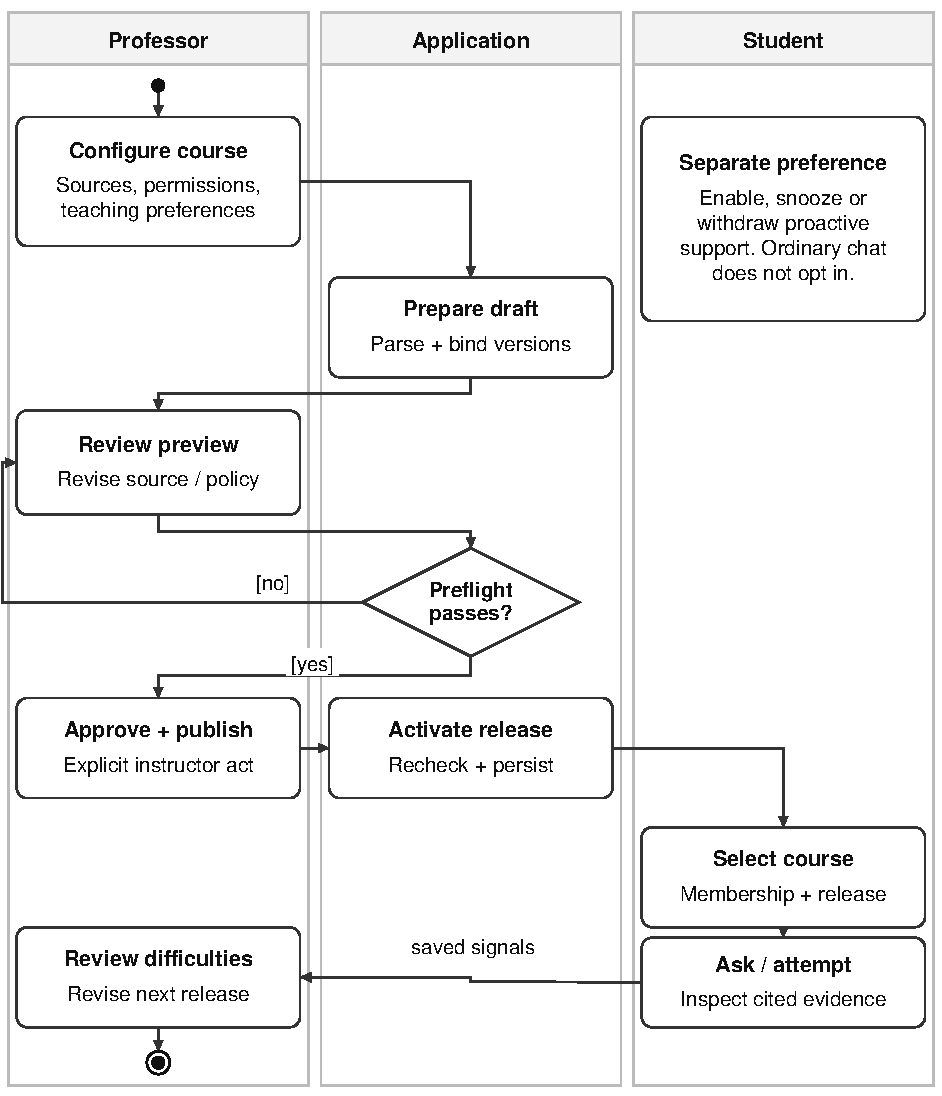
\includegraphics[width=\linewidth]{../../../reports/figures/course-twin-lifecycle.pdf}
\caption{One course configuration, publication and review cycle.}
\label{fig:lifecycle}
\end{figure}

Students select an available \emph{course}. Course membership and the published release determine which
Twin configuration the student can access. Opening a conversation associates its dialogue with that release.
A stored conversation is reused only when compatible with the current release;
withdrawn or incompatible contexts cannot authorize further tutoring.

The student asks a question, submits an attempt or opens a citation. Check-in
preferences are managed separately from ordinary chat. In the delivery workspace,
the professor can inspect goals, recorded action reasons and aggregate difficulty
signals, and pause autonomy or withdraw a release. The dashboard suppresses groups
with fewer than five learners. Its source-level difficulty summaries are signals
for instructor review, not diagnoses of individual understanding.

\subsection{From Configuration to Executable Behaviour}
The instructor's configuration has four layers (Table~\ref{tab:configuration}).
Structured action permissions restrict planning; descriptive teaching
preferences enter the configured generation pathway. The release-bound domain model maps
objectives to concepts and source evidence. Its diagnostic cues support concept
attribution, while the goal manager uses a fixed completion rule rather than
interpreting arbitrary success-condition prose.

\begin{table}[htbp]
\centering\small
\caption{Which part of the software consumes each instructor setting.}
\label{tab:configuration}
\begin{tabularx}{\linewidth}{@{}L{0.20\linewidth}Y Y@{}}
\toprule Setting & Runtime consumer & Observable effect and limit \\\midrule
Materials and permission & Ingestion, publication and retrieval & Restrict usable source versions and citation regions; upload alone does not authorize use. \\
Concepts and objectives & Attribution and goal lifecycle & Associate observed attempts with concepts; the corrected completion rule requires evidence for every concept of the exact objective. \\
Teaching preferences & Teaching-context and generation adapters & Supply tone, depth, examples and help sequence. The retained wording path is constrained; richer instruction is experimental. \\
Proactive policy & Event observer, planner and delivery service & Restrict actions and schedules; permit pause/stop. Timing, consent and frequency are checked separately from wording. \\
\bottomrule
\end{tabularx}
\end{table}

For example, the saved Socratic test profile requests a diagnostic question,
a student attempt and one hint. For the synthetic slot-seal question, its
actual first-turn response is: \emph{For \lq{}How does slot seal work\rq{}, what is
your current explanation, and which step are you unsure about?}
The response elicits an attempt but remains generic. The explanatory profile
permits a direct explanation; extracting a source rule alone does not establish
personalized progression. Appendix~\ref{sec:profile-examples} preserves the
eight-field synthetic configurations and actual response excerpts.

The instructor can also schedule support explicitly. The event-driven route
instead detects an opportunity from saved learner activity. Both routes can
reach the student without a new question. The following section explains how
observations, action selection and delivery connect, including where the
implemented connection remains approximate.

\section{Runtime Design}
\label{sec:system-design}
\subsection{Responsibilities and Persistent Data}
The architecture uses C4-style responsibility and boundary labels; interaction,
activity and state views use UML conventions~\cite{c4-notation,omg-uml251}.

The React web application presents professor and student workspaces. FastAPI
handlers~\cite{fastapi-docs} expose the operations, while domain services implement
ingestion, publication and tutoring. Repositories store courses, membership,
releases, conversations, messages, learner observations and autonomous goals.
SQLite is the local persistent store; uploaded artifacts use file-based storage.
Separate workers process ingestion and scheduled tutoring opportunities.
Figure~\ref{fig:responsibilities} shows this separation.

\begin{figure}[htbp]
\centering
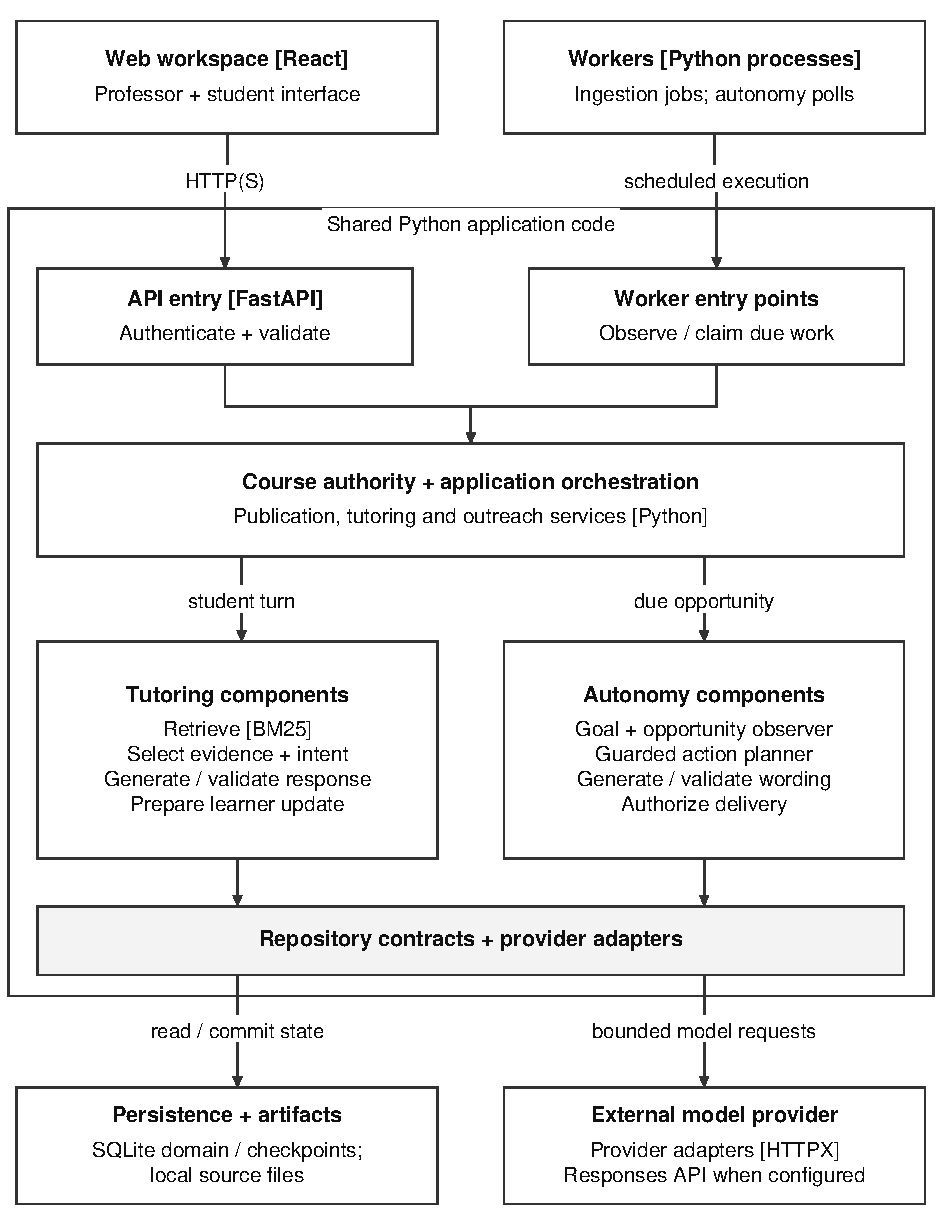
\includegraphics[width=\linewidth]{../../../reports/figures/course-twin-architecture.pdf}
\caption{Logical components shared by web requests and background workers.}
\label{fig:responsibilities}
\end{figure}

A course is owned by a professor and has student memberships. A published release
binds the policy and evidence used for tutoring. A conversation references a
course release; messages retain citations and learner observations contribute
to subsequent decisions. Autonomous goals and action outcomes also persist.
Appendix~\ref{sec:publication-data} adds publication transactions and the
conceptual persistent data model.

LangGraph provides workflow checkpoints~\cite{langgraph-docs}. Provider adapters
isolate model calls from course policy and storage. The custom OpenAI transport
uses HTTPX and the Responses API~\cite{openai-responses-docs}. Model generation
occurs outside database transactions; authority is checked again when an effect
is committed. Persisting an action requires current permission, even if a model
started generating while permission was still valid.

\subsection{From Question to Saved Response}
Figure~\ref{fig:response-sequence} traces a turn from submission to the
authorized commit of its response and learner-state update.

\begin{figure}[!ht]
\centering
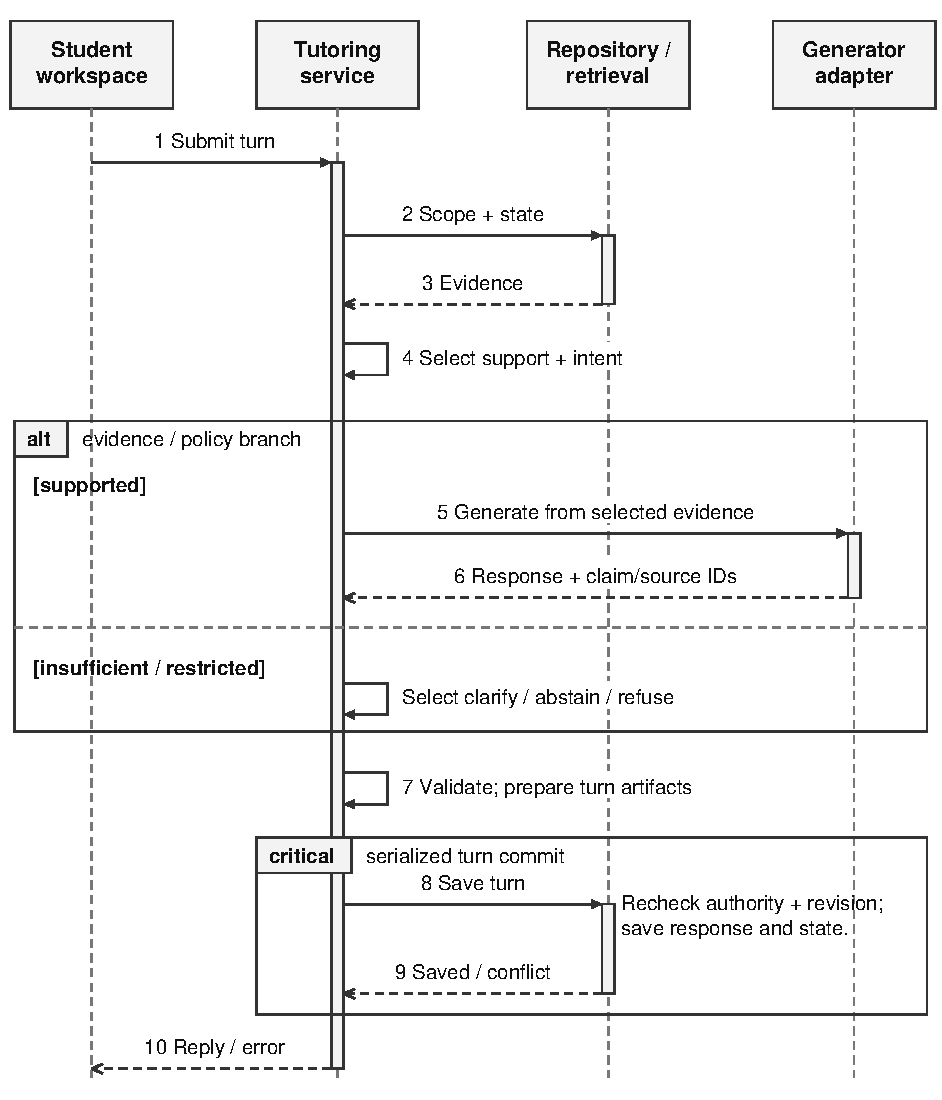
\includegraphics[width=\linewidth]{../../../reports/figures/course-twin-tutoring-sequence.pdf}
\caption{Tutoring interaction, evidence branch and serialized turn commit.}
\label{fig:response-sequence}
\end{figure}
\FloatBarrier

PyMuPDF parses approved PDFs~\cite{pymupdf-docs}; chunks preserve page boundaries,
source versions and available heading information. BM25~\cite{robertson2009bm25}
ranks eligible evidence within the student's published course. The evidence gate
checks whether support is sufficient and unambiguous. Its dominance rule
compares leading source interpretations rather than treating every weak match
as an equal competitor; competing leading answers require clarification. Retrieval and answer completeness are evaluated separately in Section~\ref{sec:grounding-comparison}.

The service validates
the account, course and release, loads policy and evidence, and invokes the
configured generation path. The retained factual path assembles approved claims
deterministically. Experimental paths ask a model for bounded explanations,
questions and feedback tied to approved source identifiers. The application
resolves citations from authoritative metadata rather than trusting invented
model links.



\begin{samepage}
After generation, current authority is rechecked within the commit boundary.
If membership, consent where applicable, or release availability has changed,
the proposed effect cannot be saved as an authorized delivery. Successful turns
persist the response, citations and associated state. A request identifier
allows matching retries to reuse the saved turn; changed content under the same
identifier is a conflict. Optimistic learner-state revision checks prevent a
stale turn from silently overwriting newer evidence.
\end{samepage}

\FloatBarrier
\subsection{From an Attempt to a Learner Record}
\label{sec:learner-state}
The observation pipeline separates identifying a concept from assessing an
answer. A turn can mention several concepts, but the primary-concept rule assigns
its assessment only to one unambiguous target; tied or weak attribution remains
unassessed. A mention therefore need not count as a correct or incorrect attempt.
The committed observation retains its concept identifiers, assessment outcome,
source references and course/release scope.

Figure~\ref{fig:learner-state} distinguishes the two consumers of stored activity.
Completion uses assessed student evidence; the default planner uses the much
simpler job-snapshot proxy. Their fields are not interchangeable.

\begin{figure}[htbp]
\centering
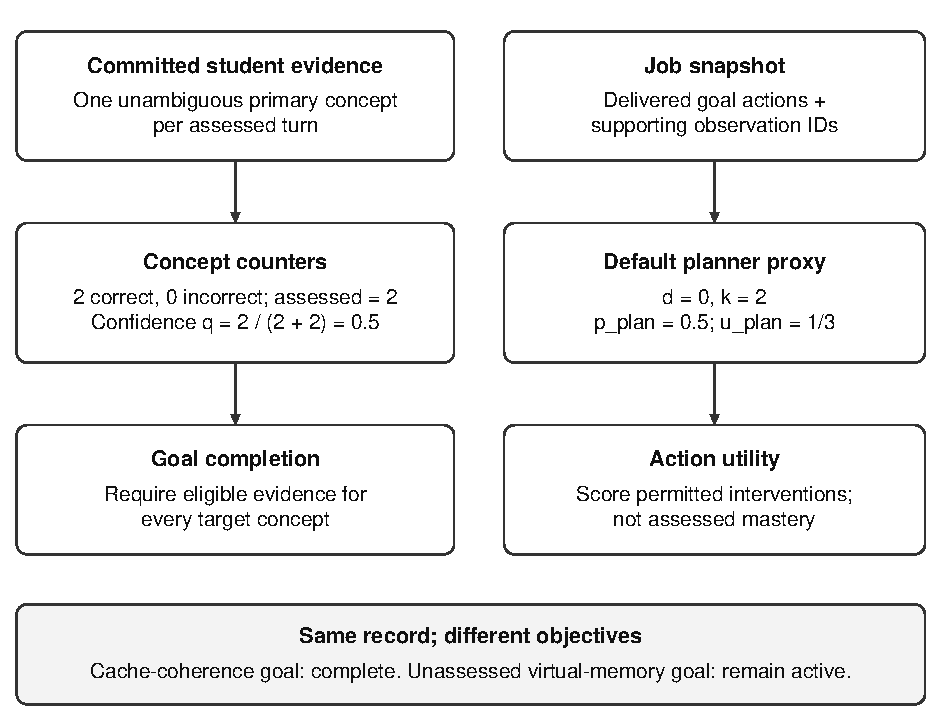
\includegraphics[width=\linewidth]{../../../reports/figures/course-twin-learner-state.pdf}
\caption{Assessment evidence and the default planner proxy have separate consumers.}
\label{fig:learner-state}
\end{figure}
For concept $c$, the evidence-count implementation records total observations,
assessed observations $a_c$, and correct, partial and incorrect counts
$(n_c^+,n_c^\sim,n_c^-)$. On an eligible assessed observation, only the relevant
outcome counter increases. Its confidence field is
\begin{equation}
q_c=\min\!\left(0.95,\frac{a_c}{a_c+2}\right).
\label{eq:evidence-confidence}
\end{equation}
Two assessed attempts give $q_c=0.5$ regardless of whether they were correct.
Thus this field represents accumulated assessment evidence, not the probability
that the student has mastered the concept. A new revision and its delta are
saved together with the accepted turn; rejected or stale observations cannot
be used as committed evidence.

The current goal correction maps each active goal $g$ to exactly one objective
in the same published domain. Let $C(g)$ be that objective's nonempty concept set,
and $S_g$ indicate that the mapping and committed learner state have valid scope.
For the evidence-count learner state, completion is
\begin{equation}
\operatorname{complete}(g)=S_g\ \land\
\bigwedge_{c\in C(g)}
\left[n_c^+\geq2\ \land\ n_c^-=0\ \land\ q_c\geq0.5\right].
\label{eq:goal-completion}
\end{equation}
Missing or ambiguous mappings remain incomplete. For example, two correct
cache-coherence assessments can satisfy a cache-coherence objective but cannot
complete an unassessed virtual-memory objective. This is the boundary reproduced
in the service audit and tested after the correction (Section~\ref{sec:goal-study}).
The rule retains a limitation: an earlier incorrect count continues to block
completion in that state. It also does not parse a professor's free-text success
condition. A completed software goal is consequently a threshold decision,
not independently demonstrated mastery.

\FloatBarrier
\subsection{How the Planner Chooses a Teaching Action}
\label{sec:planning}
The event determines candidate actions and their fallback order. Repeated
confusion permits a hint/example followed by a diagnostic question; a misconception
reverses that order. An incomplete objective or inactivity permits an in-app
check-in, and due review permits retrieval practice. The application intersects
this set with the instructor's permitted actions and adds \emph{no action}.
Let the resulting set be $A$, and $a_0$ its first permitted action.

The guarded planner scores every $a\in A$ using an inspectable forward model:
\begin{equation}
U(a)=\operatorname{clip}_{[-2,2]}
\left(G(a)+0.45O(a)+F(a)+B(a)-0.9R(a)-I(a)\right).
\label{eq:planning-utility}
\end{equation}
$G$ is a heuristic immediate-gain term weighted by estimated need and spacing;
$O$ rewards obtaining another observation when uncertainty is high; $F$ adds a
bounded look-ahead term; $B$ favours a hint or diagnostic question for repeated
errors; $R$ penalizes evidence risk and repetitive check-ins; $I$ is the
action-specific interruption cost. These constants are hand-specified, not
learned causal effects. Appendix~\ref{sec:planner-math} gives the exact terms.

Let $a^*=\arg\max_{a\in A}U(a)$, breaking ties by event order, and $a_L$
be the model proposal. Table~\ref{tab:planner-rules} makes the choice explicit;
Figure~\ref{fig:planner-decision} then applies it to the worked example.
Authorization and content validation remain separate from action selection.

\begin{table}[htbp]
\centering\small
\caption{Guarded-planner decision rules.}
\label{tab:planner-rules}
\begin{tabularx}{\linewidth}{@{}Yccccc@{}}
\toprule Condition / outcome & \shortstack{No\\evidence} & \shortstack{Invalid\\proposal} & \shortstack{Not\\best} & \shortstack{Small\\gain} & Adopt \\ \midrule
Authorized evidence ready? & N & Y & Y & Y & Y \\
Proposal valid; every step permitted? & -- & N & Y & Y & Y \\
Proposal selects analytic best ($a_L=a^*$)? & -- & -- & N & Y & Y \\
Improves fallback by at least 0.04? & -- & -- & -- & N & Y \\\midrule
Selected action & None & $a_0$ & $a_0$ & $a_0$ & $a_L$ \\
\bottomrule
\end{tabularx}
\end{table}

Ordinary provider/proposal failures retain the fallback; provider-identity errors propagate
to the failure boundary. If the model proposes the fallback itself, the action
is unchanged even though model-supplied metadata may be retained.

\textbf{What state actually reaches this planner.}
The planner receives a structured state summary, called a planning-state card.
The default adapter does not connect the detailed counts above to a calibrated
estimator. With $d$ delivered goal actions and $k$ supporting observation
identifiers, it supplies
\begin{equation}
p_{\rm plan}=\min\!\left(0.95,\frac{d+1}{d+2}\right),
\qquad u_{\rm plan}=\frac{1}{k+1}.
\label{eq:planner-proxy}
\end{equation}
The field named mastery probability therefore rises from $0.5$ to $2/3$ after
one delivery even without a student answer. Its uncertainty input counts
identifiers, not necessarily assessed attempts. Repeated-error state is derived
from the event category, and elapsed-observation time is not populated by this
adapter. These are planning proxies, distinct from Equation~\ref{eq:evidence-confidence}
and the simulator's hidden mastery. The BKT/PFA comparisons in
Section~\ref{sec:timing-comparison} are experimental alternatives, not evidence
that those estimators already drive the retained application.

\textbf{A worked calculation.}
For a repeated-confusion event with both actions permitted, zero delivered goal
actions, two supporting identifiers and ready evidence, the default adapter gives
$p_{\rm plan}=0.5$, $u_{\rm plan}=1/3$ and zero goal progress. At look-ahead
depth two, the code yields $U(\text{hint})=0.325$ and
$U(\text{diagnostic question})\approx0.267$. The event fallback is already the
hint, so a model-proposed question cannot replace it. This calculation explains
the implemented rule; it is not a recorded model response or evidence that a
hint is educationally optimal.

\begin{figure}[htbp]
\centering
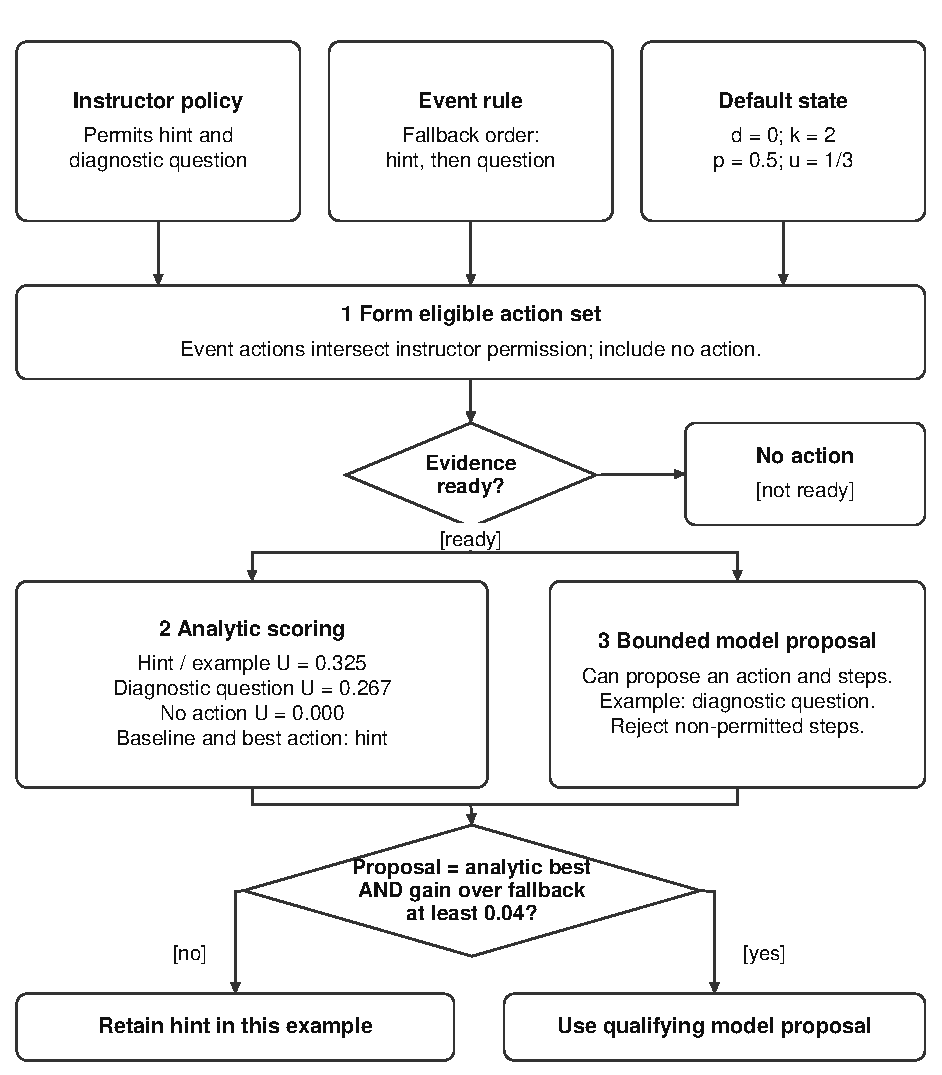
\includegraphics[width=\linewidth]{../../../reports/figures/course-twin-planner-decision.pdf}
\caption{Repeated-confusion example: the proposed diagnostic question cannot replace the higher-scoring hint.}
\label{fig:planner-decision}
\end{figure}


\FloatBarrier
\subsection{From a Durable Event to Proactive Delivery}
Autonomy here means initiating a permitted teaching action without a new
student request. A separate worker polls durable state every 30 seconds by
default. A \emph{goal} records an approved learning objective and its stopping
conditions. An \emph{opportunity} records an event, student, release and time
window in which support may be considered. An opportunity does not authorize a
message by itself.

The observer derives events from stored interactions. For example, two recent
observations with confusion scores of at least 0.7 and an overlapping concept
produce a repeated-confusion event; inactivity defaults to 72 hours without a
student message. Both thresholds are configured heuristics. Due opportunities are claimed
with a time-limited worker lease before processing.



\begin{figure}[htbp]
\centering
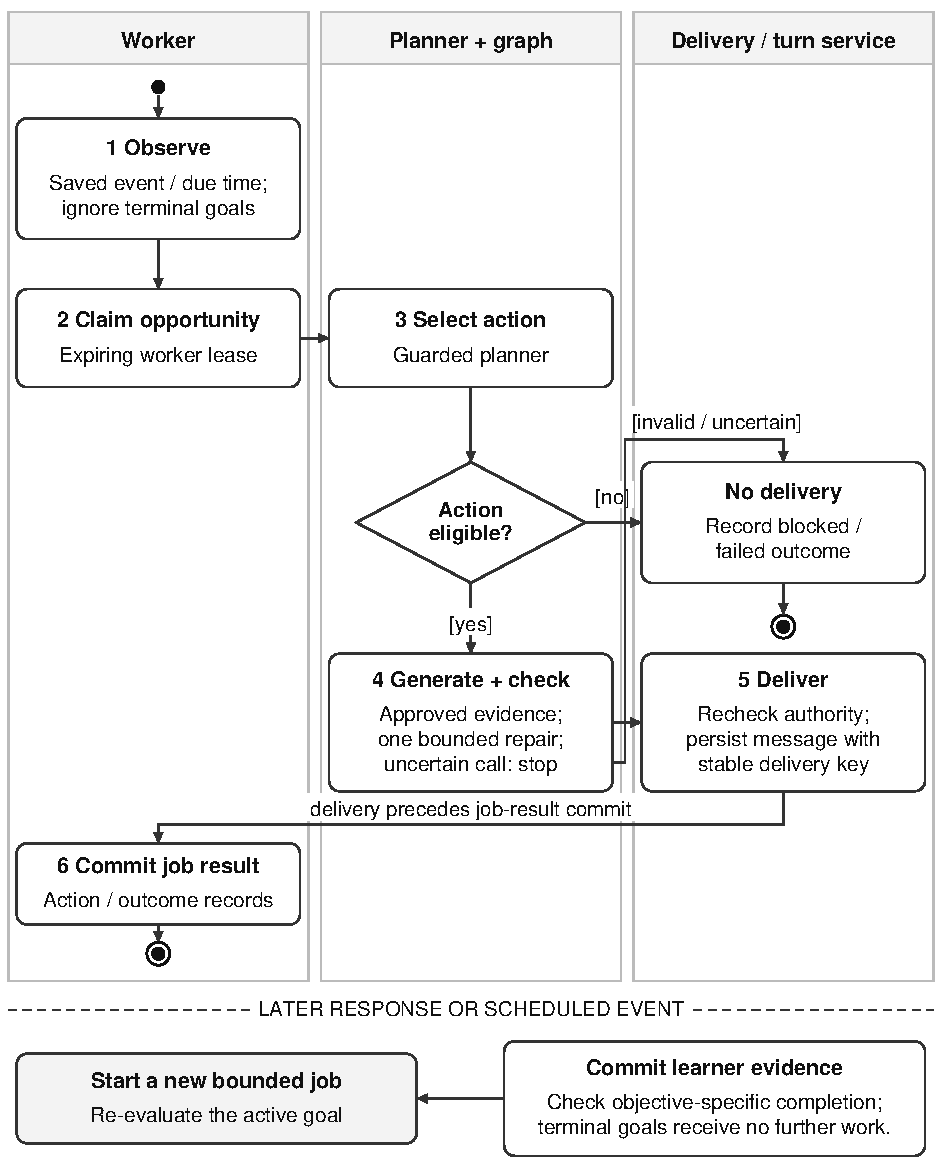
\includegraphics[width=\linewidth]{../../../reports/figures/course-twin-autonomy.pdf}
\caption{A proactive job ends after delivery or a recorded no-delivery outcome; later evidence starts another decision.}
\label{fig:autonomy}
\end{figure}

The selected model-backed wording adapter asks the model for an introduction
and a prompt strategy, then assembles permitted templates with approved source
text. Experimental instructional adapters instead generate richer questions and
explanations. 



Table~\ref{tab:outreach-decisions} specifies delivery conditions. These checks
surround a bounded graph: one proposal, initial generation and at most one repair.
An uncertain provider-call outcome stops without repeating the call. Delivery and
job-result recording are separate persistence steps; the recovery contract uses
a stable delivery key. The in-app workspace is the delivery channel.

\textbf{Following one recorded cycle.}
In the historical deterministic trace in Appendix~\ref{sec:historical-autonomy},
a diagnostic question and hint are followed by an incomplete-objective event
before the next student turn. That event leads to a permitted check-in, whose
opportunity, action and message identifiers link the decision to delivery.
Later student turns produce new learner-state revisions, and reopening the
store on virtual day 15 preserves the recorded state hash. This connects the
interaction, worker and persistence views. The trace predates the goal-completion
correction; the goal-completion regression tests that correction separately.


\begin{table}[htbp]
\centering\small
\caption{Outreach conditions and the outcome when a condition fails.}
\label{tab:outreach-decisions}
\begin{tabularx}{\linewidth}{@{}L{0.22\linewidth}Y Y@{}}
\toprule Boundary & Required condition & Otherwise \\ \midrule
Opportunity & Active and due; linked goal active and below its attempt limit & Record no action; do not generate or deliver. \\
Course authority & Consent, membership, current release/profile and instructor permission valid & Block outreach; revoked authority cannot be restored by a model proposal. \\
Schedule & Outside quiet hours; frequency and concept-cooldown checks pass & Suppress this attempt; subsequent eligible work requires a later event. \\
Evidence & Sufficient authorized support exists for the proposed action & Select no action; do not invent course evidence. \\
Generated content & Output passes the action and evidence checks & One bounded repair; stop if invalid or the provider outcome is uncertain. \\
Delivery commit & Authority still valid; stable delivery key not already saved & Reject revoked access, or reuse the already saved delivery on retry. \\
\bottomrule
\end{tabularx}
\end{table}

\subsection{A Goal Persists Across Bounded Jobs}
Figure~\ref{fig:goal-states} separates the long-lived goal from an individual
worker execution. A successful delivery increments the attempt count; it does
not complete the learning objective. The default goal manager allows three
attempts and sets expiry after seven days. The instructor may cancel a goal,
and authority changes can cancel its pending work. Pause and consent controls
prevent delivery independently of goal status. Terminal goals cannot be reactivated.

\begin{figure}[htbp]
\centering
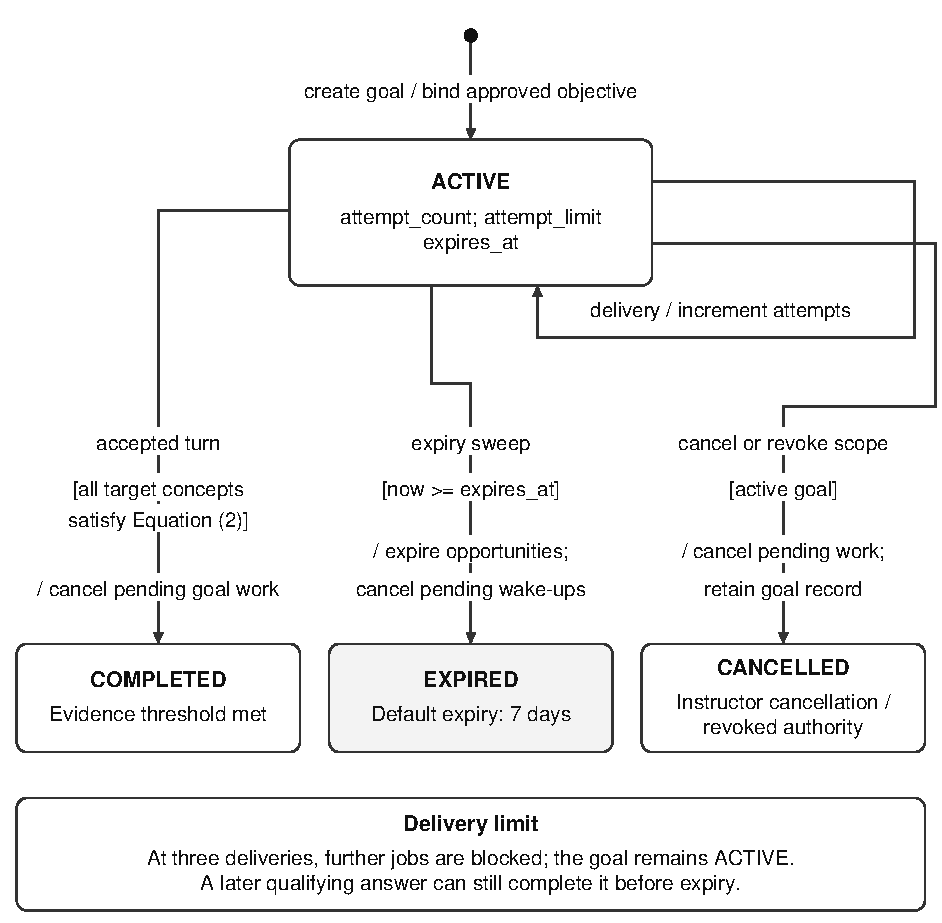
\includegraphics[width=\linewidth]{../../../reports/figures/course-twin-goal-states.pdf}
\caption{Goal transitions. Completion requires Equation~\ref{eq:goal-completion}; delivery attempts are counted separately.}
\label{fig:goal-states}
\end{figure}

\section{Comparative Evaluation and Design Decisions}
\label{sec:comparisons}
The comparisons ask which changes improve a specific software boundary.
A \emph{case} is one input, its permitted evidence and expected behaviour;
a \emph{history} contains many dependent turns for a simulated learner.
An \emph{arm} is one tested configuration. A \emph{gate} is a required acceptance condition, so a high average cannot
compensate for a critical error. The comparison names below link to exact records in
Appendix~\ref{sec:study-index}.

\begin{table}[htbp]
\centering\small
\caption{Evaluation questions, configurations and case counts.}
\label{tab:evaluation-design}
\begin{tabularx}{\linewidth}{@{}L{0.29\linewidth}Y L{0.13\linewidth}@{}}
\toprule Comparison & Cases / separation & External LLM \\\midrule
Evidence-interface comparison & 497 development cases; three extractive architectures on the same fold & No \\
Fresh factual comparison & 1,000 fresh cases; five configurations fixed before evaluation, disjoint source families & No \\
Action-planning comparison & 1,000 synthetic contexts; two configurations; 2,000 context--configuration pairs & Yes \\
Model-allocation comparison & 300 contexts; four allocations; 1,200 context--configuration pairs & Yes \\
Learner/timing simulation & 240 simulated learners per condition; nine combinations and two bounds; 30 virtual days & No \\
Revision comparison & 56 fresh scenario pairs per candidate; adequate and defective drafts & Yes \\
Live-model integration trial & 24 synthetic histories, 30 virtual days; diagnostic output review & Yes \\
Goal-completion regression & 72 histories per arm; matched seeds, exposed six-concept fixture & No \\
\bottomrule
\end{tabularx}
\end{table}

Studies use synthetic or permitted material. Only configurations within the same study
are compared directly, with shared inputs and scoring. Sample grids provide
boundary and scenario coverage. The \hyperref[study-E]{learner/timing simulation} holds out seeds within its simulator assumptions;
the \hyperref[study-H]{goal-completion regression} is a targeted regression comparison on previously exposed concepts.

\subsection{Making Retrieved Evidence Usable by the Answer Generator}
\label{sec:grounding-comparison}
\textbf{Problem and alternatives.}
A question can require two facts although its highest-ranking passage contains
only one. The evidence contract therefore needs to identify both the target
and the number of required claims. Here, an any-hit gate accepts any retrieved
passage; the typed target/cardinality interface identifies the kind and number
of facts the question requires. The \hyperref[study-A]{evidence-interface comparison} compares a lexical/any-hit control,
a typed target-and-cardinality interface, and that interface with additional
section ranking. It freezes 397 answerable and 100 boundary cases; candidate
outputs were stored before opening hidden reference answers.

\begin{table}[htbp]
\centering\small
\caption{The \hyperref[study-A]{evidence-interface comparison}: changing the evidence-to-answer contract on one development fold.}
\label{tab:evidence-interface}
\begin{tabularx}{\linewidth}{@{}Yrrr@{}}
\toprule Architecture & Grounded answers & Complete evidence@3 & Boundary action \\\midrule
Lexical/any-hit & 253/397 (63.73\%) & 95.97\% & 100/100 \\
Question type + fact count & 355/397 (89.42\%) & 98.74\% & 100/100 \\
Typed target + section ranking & 355/397 (89.42\%) & 98.74\% & 100/100 \\
\bottomrule
\end{tabularx}
\end{table}

\textbf{Interpretation and decision.}
The typed contract improved grounded success by 25.69 percentage points;
multi-evidence success rose from zero to 90.20\%. Section ranking added no
quality improvement. Remaining failures included unresolved paraphrased targets,
neighbouring source regions and extracted claims that missed the required span.
The typed interface was retained as the next development baseline, with
\emph{Refine} status: no arm passed every quality gate. 

\paragraph{How factual success is scored.}
For answerable case $i$, $g_i=1$ requires the correct answer action, all required
answer spans, exact claim/citation coverage, valid source versions and no
operational failure. Otherwise $g_i=0$. Claim/citation precision and recall must
both equal one. For boundary case $j$, $b_j=1$ requires the expected
clarification, abstention or refusal action. In the \hyperref[study-B]{fresh factual comparison},
\begin{equation}
\begin{aligned}
\text{Grounded success}&=\frac{100}{N_A}\sum_i g_i
 =100\frac{506}{800}=63.25\%,\\
\text{Boundary accuracy}&=\frac{100}{N_B}\sum_j b_j
 =100\frac{192}{200}=96\%.
\end{aligned}
\label{eq:grounded-score}
\end{equation}
Missing a required second fact fails the whole case. Normalized text and source-range matching
make the scorer inspectable but do not provide unrestricted semantic grading.

Let $E_i$ be the required evidence items and $M_i(3)$ those matched within the
first three results under the source/version/range rules. Then
\begin{equation}
\text{Complete evidence@3}
=\frac{100}{N_A}\sum_i\mathbf{1}[M_i(3)=E_i].
\label{eq:retrieval-score}
\end{equation}
Retrieval can score one while an incomplete answer scores zero. The \hyperref[study-B]{fresh factual comparison}'s
retained BM25 configuration with the dominance gate retrieved complete evidence in 98\% of
answerable cases but delivered only 63.25\% fully grounded answers. Its
family-bootstrap 95\% interval was 58.75--67.63\%, resampling the 200 source
families 10,000 times rather than treating related questions as independent.
The hybrid arm with the same gate scored 62\%. BM25 was retained as the simpler local
fallback; both failed factual acceptance.

The \hyperref[study-B]{fresh factual comparison}'s any-hit control had zero cases satisfying the complete grounding rubric despite 98\% retrieval
coverage: it passed an unrestricted evidence set to a generator requiring one
or two selected claims. This incompatible composition differs from the \hyperref[study-A]{evidence-interface comparison}'s lexical
control. The dense/hybrid arms use the Qwen embedding model~\cite{qwen3-embedding-card}.

\subsection{What the 10,000-Case Tests Revealed}
\label{sec:large-regression}
The large tests answer a different question from the fresh 1,000-case comparison:
does a selected composition still behave correctly when a course contains many
potentially competing source regions? Three records must be distinguished. The pipeline-scale test's later correction is separately
indexed as \hyperref[study-L1c]{pipeline-test correction}.

\begin{table}[htbp]
\centering\small
\caption{Large-test evidence and its limits. The whole-corpus regression reuses the large product test's known corpus; it is
not fresh generalization evidence. A 1,000-case control is a subset comparison,
not an additional 1,000 independent questions.}
\label{tab:large-tests}
\begin{tabularx}{\linewidth}{@{}L{0.22\linewidth}L{0.24\linewidth}Y@{}}
\toprule Test & Execution unit & What the record supports \\ \midrule
\hyperref[study-L1]{pipeline-scale test} & 10,000 cumulative pipeline cases & Processing and validation completed. Later audit found that the authoring path saw the reference answer and supplied its answer/citation; it did not independently test product retrieval and generation. \\
\hyperref[study-L2]{large product test} & 10,000 product cases; 1,000 paired controls & 8,000 answerable and 2,000 boundary cases; product received the course and question before hidden scoring. Recorded 478 severe unsupported releases and 594 operational failures; release-quality gates failed. \\
\hyperref[study-L3]{whole-corpus regression} & Same known 10,000 cases; 1,000 paired controls & Deterministic ambiguity-checking candidate; no external LLM calls. Recorded four severe unsupported releases, zero operational failures and 6,973 clarifications. Eleven of sixteen gates failed. \\
\bottomrule
\end{tabularx}
\end{table}

The large product test reported pooled grounded success of 44.16\%. Its
hierarchical source-family estimate was 42.94\% (95\% interval
41.03--44.96\%); the interval belongs to that estimate, not the pooled rate.

\textbf{Failure mechanism.}
The original ambiguity gate compared distinct answer meanings across every candidate
above a coverage threshold. In a full course, a weaker region could therefore
compete with the strongest relevant answer. Earlier confirmation published only
one approved chunk per release, so this ambiguity branch could not fire.
Figure~\ref{fig:evidence-failure} explains why passing that confirmation did
not establish corpus-scale behaviour. The 100-case diagnostic found the target
region ranked first in 84 cases, with 69 of those still returning clarification.
This motivated comparing dominant interpretations rather than all weak matches.
The subsequent fresh factual comparison remains the evidence for the retained fallback;
its quality gates also failed.

\textbf{Unresolved numerical inconsistency.}
The whole-corpus regression's durable summary labels 25.38\% as fully grounded factual success over
8,000 answerable cases, but separately records only 1,669 answer actions in all
10,000 cases. Under the scorer's requirement of a correct answer action, the
upper bound from that action count is $1669/8000=20.86\%$. These fields cannot
both describe the same scored ledger. The original record is preserved; the
25.38\% value is excluded from performance comparisons pending reconciliation
with the original per-case ledger, which was not located in the inspected
local evidence. The failure diagnosis and recorded
gate dispositions are reported as such, without turning that percentage into
a validated accuracy claim.

\begin{figure}[htbp]
\centering
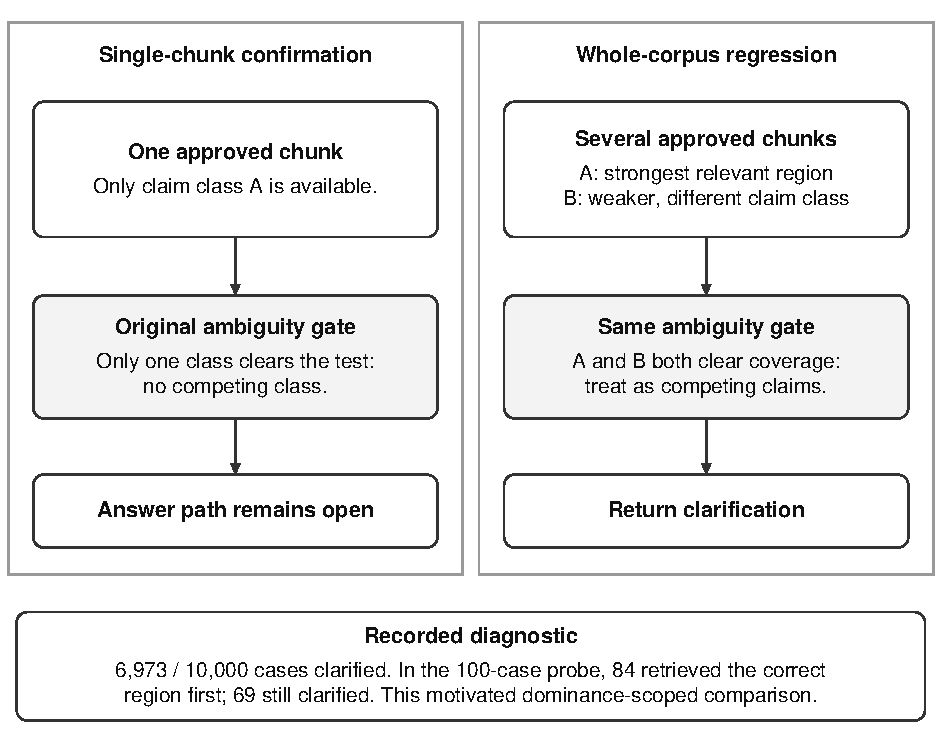
\includegraphics[width=\linewidth]{../../../reports/figures/course-twin-evidence-failure.pdf}
\caption{Original ambiguity checks under single-chunk and whole-corpus inputs (Whole-corpus regression).}
\label{fig:evidence-failure}
\end{figure}

\subsection{Selecting Actions and Allocating Models}
\label{sec:planner-comparison}
\textbf{Problem and alternatives.}
The planner must use model proposals without allowing malformed or unsuitable
proposals to suppress a valid baseline action. Earlier fixed-rule, model-only,
hierarchical and reject-only-verifier trials led to the guarded design.
The \hyperref[study-C]{action-planning comparison} then compared that design with the deterministic workflow on 1,000
synthetic contexts. These component trials supply explicit planning-state cards;
they do not validate the default product adapter's delivery-count proxy.

\begin{table}[htbp]
\centering\small
\caption{Action-planner results on 1,000 shared contexts.}
\label{tab:planner-comparison}
\begin{tabularx}{\linewidth}{@{}Yrrrr@{}}
\toprule Planner & Valid action & Preferred & Utility & Regret \\\midrule
Deterministic workflow & 100\% & 74\% & 0.7954 & 0.0129 \\
Guarded policy-value & 100\% & 73\% & 0.8002 & 0.0081 \\
\bottomrule
\end{tabularx}
\end{table}

Here, evaluation utility is the synthetic instrument's registered action value,
using the public state card and a seeded hidden learner outcome. For example,
not knowing the concept adds value to diagnostic support or a hint, and the
event type supplies an action-specific bonus. Mean regret is the difference
from the highest-valued permitted action.
Preferred-action agreement checks a separate reference label. Neither is
measured student learning, and this evaluation utility must not be confused
with the runtime heuristic $U$ in Equation~\ref{eq:planning-utility}.
The positive paired utility improvement replicated while hard gates held,
so the guarded planner advanced to engine comparison. Preferred agreement fell
by one percentage point; the result supports a conditional design choice,
not improvement on every definition of appropriate action.

The \hyperref[study-D]{model-allocation comparison} holds the architecture fixed and crosses two planner models with two
wording models. Table~\ref{tab:model-allocation} shows the complete four-way
comparison. The alternative planner's pooled utility effect was $+0.000354$
(95\% interval $0$--$0.001062$). The alternative wording model's valid-strategy
effect was $+0.00417$ ($0$--$0.01042$). Neither satisfied the preregistered rule requiring the entire interval to exceed zero. The Terra-planner/Luna-wording combination also missed the 99.5\% generator-completion gate
at 238/240 calls; its two failures used the deterministic fallback.

\begin{table}[htbp]
\centering\small
\caption{The \hyperref[study-D]{model-allocation comparison}: model allocation under one guarded architecture.
Luna and Terra denote GPT-5.6 variants; Mini is GPT-5.4 Mini (2026-03-17).}
\label{tab:model-allocation}
\begin{tabularx}{\linewidth}{@{}YYrr@{}}
\toprule Planner & Wording & Utility & Valid final wording \\\midrule
Luna & Luna & 0.7935 & 100\% \\
Terra & Luna & 0.7938 & 100\% \\
Luna & Mini & 0.7935 & 100\% \\
Terra & Mini & 0.7938 & 100\% \\
\bottomrule
\end{tabularx}
\end{table}

The Luna-planner/Luna-wording combination was the simplest and least expensive eligible allocation under the recorded
rule and advanced to whole-system confirmation. Valid final wording includes
fallback behaviour; it does not imply every provider call succeeded. 

\subsection{Combining Learner Estimation with Intervention Timing}
\label{sec:timing-comparison}
\textbf{Problem and alternatives.}
Sending fewer reminders can reduce waste while also removing useful practice.
The \hyperref[study-E]{learner/timing simulation} separates the estimate of need from the decision to intervene. It
crosses a count baseline, Bayesian Knowledge Tracing (BKT) and Performance
Factors Analysis (PFA) with constant, conditional and value-based timing.
BKT updates a latent knowledge estimate from observed performance
\cite{corbett1994knowledge}; PFA relates performance to prior successful and
unsuccessful practice~\cite{pavlik2009performance}. The local variants include forgetting/decay.

Figure~\ref{fig:simulation-design} shows the development/held-out split and
which information the candidates can observe. The simulation does not execute
text retrieval or generation. The two bounds locate the comparison between
never intervening and using simulator knowledge unavailable to the candidates.

\begin{figure}[htbp]
\centering
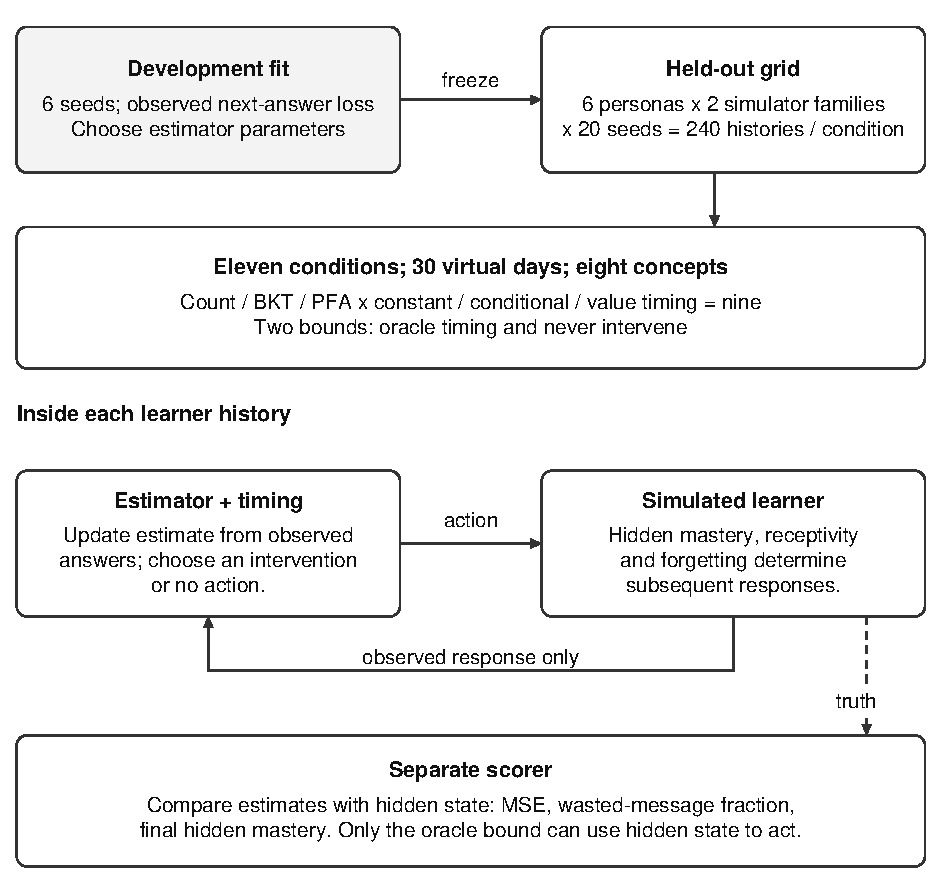
\includegraphics[width=\linewidth]{../../../reports/figures/course-twin-simulation-design.pdf}
\caption{Learner/timing simulation: held-out comparison with separate observation and scoring inputs.}
\label{fig:simulation-design}
\end{figure}

\begin{table}[htbp]
\centering\small
\caption{The \hyperref[study-E]{learner/timing simulation}: all nine estimator/timing combinations and two bounds.
Mean squared error (MSE) and waste are lower-is-better; mastery is a simulator state on $[0,1]$.
Messages and rates are means over 240 learners per condition.}
\label{tab:learner-timing}
\begin{tabularx}{\linewidth}{@{}Yrrrr@{}}
\toprule Estimator + timing & MSE & Messages & Waste & Final mastery \\\midrule
Count + constant (baseline) & 0.084 & 14.0 & 50.6\% & 0.314 \\
Count + conditional & 0.084 & 7.0 & 38.8\% & 0.302 \\
Count + value & 0.084 & 10.2 & 34.1\% & 0.317 \\
BKT + constant & 0.035 & 14.0 & 46.4\% & 0.317 \\
BKT + conditional & 0.035 & 8.9 & 36.6\% & 0.309 \\
BKT + value & 0.037 & 12.3 & 30.1\% & 0.328 \\
PFA + constant & 0.052 & 14.0 & 50.8\% & 0.313 \\
PFA + conditional & 0.051 & 7.3 & 41.5\% & 0.303 \\
PFA + value & 0.051 & 10.5 & 34.7\% & 0.313 \\\midrule
Count + oracle (bound) & 0.086 & 12.2 & 0.0\% & 0.345 \\
Count + never (bound) & 0.083 & 0.0 & -- & 0.288 \\
\bottomrule
\end{tabularx}
\end{table}

For daily concept estimate $\hat m_{hct}$ and simulator truth $m_{hct}$,
MSE averages $(\hat m_{hct}-m_{hct})^2$ over concept-days within each history
$h$, then across histories. A delivered intervention is labelled wasted when
the simulator says the learner is unreceptive or already has mastery at least
$0.85$. Waste is the mean of per-history wasted-delivery fractions, not a
human rating of the message. Final mastery averages hidden concept states on
day 30. The simulator defines all three quantities.

\begin{samepage}
\textbf{Interpretation and decision.}
BKT with value-based timing reduced waste by 20.5 percentage points relative
to count/constant (95\% paired-bootstrap interval $-22.8$ to $-18.3$ points).
Its final simulated mastery increased by $0.014$ ($0.007$--$0.021$), using
1,000 learner-level paired resamples. Count/conditional halved delivery but
reduced final mastery by $0.012$ ($-0.018$ to $-0.005$). Thus suppressing
messages alone did not deliver the best trade-off.
\end{samepage}

Hidden-state MSE improved, but BKT's next-answer Brier-score difference under
constant timing was inconclusive ($-0.00027$, 95\% interval $-0.00630$ to
$0.00552$). The initial attempt was invalidated because one
simulator's forgetting overwhelmed learning; its result and the corrected
attempt remain archived. The decision was \emph{Go Deeper}: retain BKT/value
as a hypothesis, with PFA as comparator. Integration with the product's
committed observations, a decayed-count control and a third simulator family
have not yet been completed. 

\subsection{Richer Instruction, Revision and Visual Evidence}
\textbf{Problem and alternatives.}
Constrained source assembly protects factual provenance but can produce generic
questions. Typed instructional units and bounded revision were evaluated to
allow more useful explanations while retaining source authority. A typed
instruction candidate was rated useful on 44/48 evaluated targets by assistant
review, compared with 16/48 for the control. These are rubric targets rather
than independent student judgments. The candidate retained one critical
attribution error. In the fresh \hyperref[study-F]{revision comparison}, each of two revision candidates received
56 adequate/defective scenario pairs. Both preserved 56/56 adequate drafts
and repaired 47/56 defective drafts (83.9\%), but each retained one critical
error. A cited necessary condition was treated as sufficient. Both failed
the zero-critical-error gate and remained unpromoted.

The reference answers were authored and cross-reviewed before candidate outputs were generated, and
uncertain judgments remained in the denominator. Nevertheless, the scoring
process was AI-assisted. Earlier source-oracle corrections and later response
audits that missed known critical errors show why structural validity and
citations do not establish semantic correctness. These failures are retained
alongside successful controls in the repository result records.

Visual experiments tested whether images supplied evidence that text lost.
In the historical comparison using the Jina embeddings v4 visual model~\cite{jina4-card}, relevant visual retrieval
improved from 18/30 to 28/30, yet both product arms achieved only 20/30 grounded
answers, and both retained critical citation failures. In a separate fresh comparison using the Jina embeddings v5 omni model~\cite{jina5-card},
the candidate achieved 16/30 grounded answers versus 26/30 for its text/OCR
control. Source-region lineage and packet layouts remained failure points;
the control also retained a citation defect. The omni candidate was dropped.
The selected product parser accepts selectable PDF text; general scanned-PDF
OCR remains unqualified.


\section{Selected Composition and Integrated Verification}
\label{sec:verification}
\subsection{What Was Selected, and What Remains Experimental}
The local final manifest selects BM25 retrieval, ambiguity-aware evidence
selection, deterministic factual assembly, guarded model planning and persistent
in-app outreach. The exact profile is listed in Appendix~\ref{sec:software}. Table~\ref{tab:design-decisions} distinguishes
comparison-based choices from requirements that the implementation must enforce.

The experiments do not identify a single composition that wins on every
criterion. The evidence-interface comparison tests a development evidence interface; the fresh factual comparison supports
the retained factual fallback. The action-planning and model-allocation comparisons compare planners using supplied
state cards, whereas the product adapter still supplies delivery/event proxies.
The learner/timing simulation evaluates estimator/timing alternatives outside the tutoring service.
The live-model integration trial exercises an integrated development configuration with actual model
calls, and the goal-completion regression isolates a later lifecycle correction without model calls.
Thus neither the component improvements nor the historical integrated run
constitute an end-to-end qualification of all current components together.


\begin{table}[htbp]
\centering\small
\caption{Current disposition of the principal designs.}
\label{tab:design-decisions}
\begin{tabularx}{\linewidth}{@{}L{0.23\linewidth}Y Y@{}}
\toprule Design boundary & Current disposition & Basis and unresolved issue \\\midrule
Source/policy binding & Retain reviewed, immutable releases & Required for authority and reproducible dialogue; supported by publication tests, not a performance ranking. \\
Retrieval and factual wording & Retain BM25/dominance and deterministic assembly & The \hyperref[study-B]{fresh factual comparison} supports the simpler local fallback, not a qualified winner; grounded and boundary scores remain below targets. \\
Question-to-evidence mapping & Retain as development design & The \hyperref[study-A]{evidence-interface comparison} improves coverage; not all gates pass and not a release-wide 89.42\% claim. \\
Autonomous planning/wording & Retain guarded planning with Luna for both planning and wording & Synthetic utility supports progression to integration, despite lower preferred-action agreement; product proxy inputs and individualized instruction remain unvalidated. \\
Learner estimator/timing & Keep current evidence counters; BKT/value remains experimental & The \hyperref[study-E]{learner/timing simulation} supports further work, but its estimator is not wired into the default planning adapter. \\
Goal lifecycle correction & Keep objective-scoped completion in the working tree & The \hyperref[study-H]{goal-completion regression} removes unsupported completions; full frozen-release requalification is separate. \\
Flexible generation and vision & Keep unsuccessful candidates as development evidence & Critical semantic/attribution failures or no end-to-end gain prevented promotion. \\
Delivery and persistence & Retain leased jobs, authority rechecks and stable delivery keys & Required for consent and restart behaviour; local operational checks bound the evidence. \\
\bottomrule
\end{tabularx}
\end{table}

The selected profile uses GPT-5.6 Luna for bounded complex planning and wording
strategies. Flexible instructional trials are separate configurations. Likewise,
the current objective-scoped correction postdates the frozen local qualification:
its experimental component profile and matched regression study support that
correction, not a claim that the complete final release was requalified.

\subsection{Thirty Virtual Days with Actual Model Calls}
\label{sec:provider-study}
The \hyperref[study-G]{live-model integration trial} executes the integrated development composition over 24 synthetic
histories and 30 virtual days. It uses actual external LLM calls for its
configured model pathways: 654 calls were recorded, 643 completed and 11
reached the output limit. The run processed 484 tutor turns, delivered 16 proactive
messages and exercised 24 service restarts. Consent was disabled on virtual
days 10--19; no proactive messages were delivered in that interval.

The software actually executed dialogue processing, persistent learner records,
autonomous jobs, delivery and restart recovery. Student utterances, attendance and receptivity were synthetic, and time
advanced virtually. This operational trial did not score changes in mastery
and does not establish 30 days of uptime. The separate learner/timing simulation
and goal-completion regression make no external model calls; they examine
simulated learning mechanisms and state-management correctness, respectively.

Thirteen tutoring turns ended in a safe graph failure, including two invalid
question-focus selections. A post-run AI diagnostic reviewed 48 endpoint
responses, all 13 failures and all 16 check-ins: 77 deliberately selected cases,
not a representative estimate of response quality. All 16 check-ins used a
generic wrapper around an entire source card; their effect on students was
not measured. In the saved Socratic first-turn
case, the tutor asks for the student's current explanation but does not make
the question specific to the concept's underlying difficulty
(Appendix~\ref{sec:profile-examples}).

The operational finding is that the composed software can initiate and preserve
support under the tested controls. The instructional finding is narrower:
successful authorization and delivery did not ensure a useful, personalized
question. Provider cost, latency and the precise historical configuration remain
in the linked study record (Appendix~\ref{sec:study-index}).

\subsection{A Goal-Completion Defect and Its Revision Cycle}
\label{sec:goal-study}
A service reproduction exposed a missing invariant: completing goal $g$ must
depend on evidence for $C(g)$, not the strongest concept anywhere in the learner
record. With cache-coherence and virtual-memory goals active, two correct
cache-coherence attempts incorrectly completed both goals; reopening SQLite
preserved the error. The old service shortcut and goal interpreter both used
evidence too broadly.

The revised design applies Equation~\ref{eq:goal-completion} separately to each
goal and accepts only committed state from the relevant scope. Multi-goal and
multi-concept regressions cover missing, unrelated, incorrect, ambiguous and
uncommitted evidence, plus restart and continued work on another goal. The
prospective \hyperref[study-H]{goal-completion regression} then compares the old and corrected implementations.
Only two runtime source files differ between the archived arms; the driver,
six concepts, seeds, profiles and dependencies match.

Each arm runs 72 histories: six personas, two simulator families, three seeds
and reactive/autonomous conditions, with a restart on virtual day 15. The
product service, worker and SQLite paths execute; wording and planning are
deterministic. Shared initial conditions and seeds do not imply identical
later transcripts, because changed interventions can change simulated replies.

\begin{table}[htbp]
\centering\small
\caption{The \hyperref[study-H]{goal-completion regression}: matched lifecycle correction, 72 histories per arm.
The last two rows concern the 36 autonomous histories per arm.}
\label{tab:goal-correction}
\begin{tabularx}{\linewidth}{@{}Yrr@{}}
\toprule Measure & Original & Objective-scoped \\\midrule
Completed goals & 26 & 15 \\
Supported by target concepts & 14 & 15 \\
Unsupported completion & 12 & 0 \\
Histories with unsupported completion & 11 & 0 \\
Consistent restarts & 72/72 & 72/72 \\
Attribution / assessment agreement & 100\% / 100\% & 100\% / 100\% \\
Quiet-hour / frequency / cooldown violations & 0 / 0 / 0 & 0 / 0 / 0 \\\midrule
Mean proactive messages & 9.056 & 10.611 \\
Mean final simulated mastery & 0.3632 & 0.3608 \\
\bottomrule
\end{tabularx}
\end{table}

The old assessment gates passed even when goal completion was wrong. The
corrected arm passed all 19 run gates. Target-supported completions numbered
14 in the original arm and 15 in the corrected arm; unsupported completions
numbered 12 and zero. Total completed goals measure software status decisions,
not student learning success. A separate audit matches each completion to committed
target-concept evidence. Equal virtual timestamps cannot establish exact commit
ordering, so service regressions separately test that boundary.

The correction increased proactive delivery by 56 messages across the autonomous
histories. Mean simulated mastery changed by $-0.0024$, and mean wasted-message
fraction rose from $0.3496$ to $0.3572$. The evidence supports \emph{Keep} for
objective-scoped state correctness. The mastery difference is a descriptive
secondary outcome relative to the previous implementation, not a measurement
of learning effects in students. Eleven autonomous histories increased, nine
decreased and sixteen were unchanged. This regression uses previously exposed
concepts.

A retrospective audit of the earlier 72-history multi-concept trial
found ten unsupported completions among 22 completed goals in eight histories.
Its original measurements and prior successful assessment correction are
retained, but they cannot establish correctness of the now-revised lifecycle.
The four completed goals in the \hyperref[study-G]{live-model integration trial} showed no such mismatch; that small audit
does not qualify all provider-backed paths. Appendix~\ref{sec:historical-autonomy}
preserves the original simulated outcome and its later interpretation.

\subsection{Verification and Acceptance Boundaries}
This revision cycle supplies a concrete software development lifecycle (SDLC) argument: reproduce the defect,
state the missing invariant, change the responsible boundary, compare the
implementations, and retain both the failed baseline and bounded acceptance.
The focused service/component/audit suite passed 72 tests, including 30 new
regressions. The broader Python run and its targeted rechecks are documented in
Appendix~\ref{sec:sdlc}; they are not a single clean post-correction full run.

For course configuration and human control, browser diagnostics exercised preview, approval, reload and
withdrawal. Local qualification recorded 43 application checks and 51 container
regressions; restart, restore and rollback were tested under that environment.
These support publication and operational contracts. They do not replace factual acceptance, pedagogical review or real-course
validation of continuing support.
At submission, course configuration and human control have bounded local
verification; factual support remains below acceptance targets; teaching-style
alignment lacks validation with the actual instructor; and continuing support
has operational and lifecycle evidence but not demonstrated learning
benefit. The prototype implements the course and tutoring workflows, but has not met
all five acceptance requirements: factual-quality gates remain unmet, and
instructor fidelity and real-student learning effects remain unvalidated.

\section{Findings, Limitations and Next Decisions}
The project connects instructor configuration to course-grounded responses and
proactive support through explicit evidence, state and execution contracts.
The comparison results identify three engineering findings. First, the
evidence-to-generator interface can matter more than increasing retrieval
complexity: typed targets improved a development comparison, while additional
ranking did not. Second, guarded planning and model allocation should be judged
against their stated objective: utility improved in the planner comparison
without improving every action label. Third, operational correctness and
instructional usefulness diverge: delivered, persistent check-ins can remain
generic. The objective-scoped correction improved completion correctness but
did not increase mean final simulator mastery relative to the old logic.

Flexible instruction, visual
retrieval and BKT/value timing have different development statuses. In
particular, the default planner still consumes delivery/event-based proxies
rather than a calibrated model of the committed learner evidence. The
objective-scoped completion correction addresses a real defect but retains
fixed thresholds and cumulative contradiction handling.

Validity is limited by synthetic courses, mechanical questions, simulator
assumptions and shared AI involvement in construction and review. Some
historical trials retain aggregates but lack the original per-case artifacts;
the appendix records those gaps rather than reconstructing evidence. Local
tests and virtual time do not establish production-scale uptime. The evaluations did not include an approved study with the actual instructor
or real students; those outcomes remain untested.

The next design decision is to compare a planner adapter based on committed
concept evidence against the present proxy, while retaining a simple control.
That comparison should then be integrated with source-supported,
profile-sensitive question generation and independently reviewed assessment.
An approved course pilot would test usefulness and student experience after
those gates. 
\section*{Declaration of AI Assistance}
\label{sec:ai-assistance}
OpenAI Codex assisted research planning, implementation, evaluation design and
analysis, synthetic cases and reference answers, literature and reference checking,
figures, and report drafting and revision. This assistance is distinct from the
model APIs evaluated in the system. AI-reviewed results are labelled and are not
independent human assessment. The author is responsible for the work, source
attribution and interpretation.

\clearpage
\bibliographystyle{unsrtnat}
\bibliography{references}
\clearpage
\appendix
\section{Failure Mechanisms and Design Disposition}
\label{sec:failure-map}
\label{sec:design-summary}
\begin{table}[htbp]
\centering\small
\caption{What failed, the observed mechanism and the resulting engineering decision.}
\begin{tabularx}{\linewidth}{@{}L{0.19\linewidth}Y Y@{}}
\toprule Design / evidence & Failure mechanism & Disposition and remaining limit \\\midrule
Any-hit evidence gate; factual confirmation & The generator expected one or two selected claims; the gate passed an unrestricted set. Correct retrieval therefore ended in abstention. & Preserve as a failed interface control. Use question-targeted selection and ambiguity checks; 63.25\% still fails complete-answer acceptance. \\
Dense/hybrid retrieval; same factual set & Higher complexity did not improve downstream scores: 62\% versus BM25's 63.25\%.  & Retain BM25 locally.  \\
Visual retrieval; omni confirmation & Candidate failures concentrated in packet layouts and source-region attribution: 16/30 grounded and 16/30 original-region lineage. & Drop this candidate. The 26/30 text/OCR control also had a wrong-region/invalid citation; visual capability remains limited. \\
Instruction and revision; fresh paired drafts & Source-linked wording could assert sufficiency from a necessary condition. Both revision candidates preserved 56/56 drafts and repaired 47/56, but each retained one critical failure. & Do not promote based on aggregate repair rate. Validate the delivered claims, including supplementary examples. \\
Learner assessment; multi-concept correction & One assessment spread across weak concept matches. Primary-concept-only assignment corrected that attribution problem. & Keep concept-assessment correction. The later goal audit found 10 unsupported completions in this historical run; the new paired lifecycle study removes that defect. Prediction and teaching remain separate. \\
Goal completion; the \hyperref[study-H]{goal-completion regression} & The strongest concept's evidence completed unrelated goals. Both the service shortcut and interpreter lacked target-specific binding. & Require every concept of the exact objective. Unsupported completions fell from 12 to zero; mean final simulator mastery changed by $-0.0024$ relative to the old logic. \\
Model-backed outreach; saved dialogue & All 16 reviewed check-ins wrapped an entire source card in generic guidance. Permission checks did not assess instructional usefulness. & Retain operational evidence only; contextual progression needs separate evaluation. \\
Evaluation oracle; corrected controls & A source/reference packet reversed a one-way implication; structural checks did not detect every semantic defect. & Preserve invalid and corrected records. AI review is diagnostic; quality claims need independently checked reference meaning. \\
\bottomrule
\end{tabularx}
\end{table}

The linked evidence index in Appendix~\ref{sec:study-index} identifies the
source records. Historical attempts remain in the repository, including
invalid results and subsequent corrections. \clearpage
\section{Publication and Data Relationships}
\label{sec:publication-data}
Figure~\ref{fig:data-detail} identifies the persistent relationships used by
publication and tutoring.
\begingroup
\setlength{\intextsep}{3pt}
\setlength{\abovecaptionskip}{4pt}
\begin{figure}[!ht]
\centering
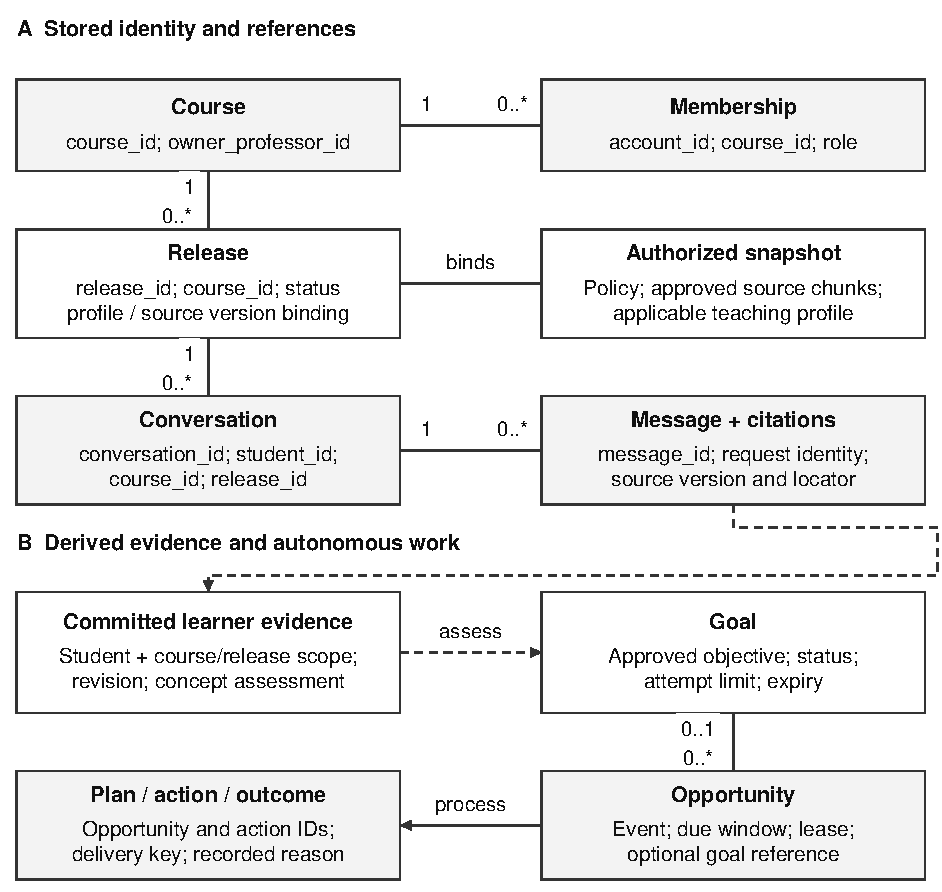
\includegraphics[width=\linewidth]{../../../reports/figures/course-twin-data-relationships.pdf}
\caption{Conceptual relationships among course releases, conversations, learner evidence and autonomous work.}
\label{fig:data-detail}
\end{figure}
\FloatBarrier
\endgroup
\clearpage
Publication is a separate state transition from preview or preflight.
Figure~\ref{fig:publication-detail} shows both operations and their failure
boundary. The preflight records deterministic readiness checks; it does not
replace the academic quality evaluations in the results section. The observer
runs after publication commits. Rollback revalidates and republishes a withdrawn release.
\begin{figure}[!ht]
\centering
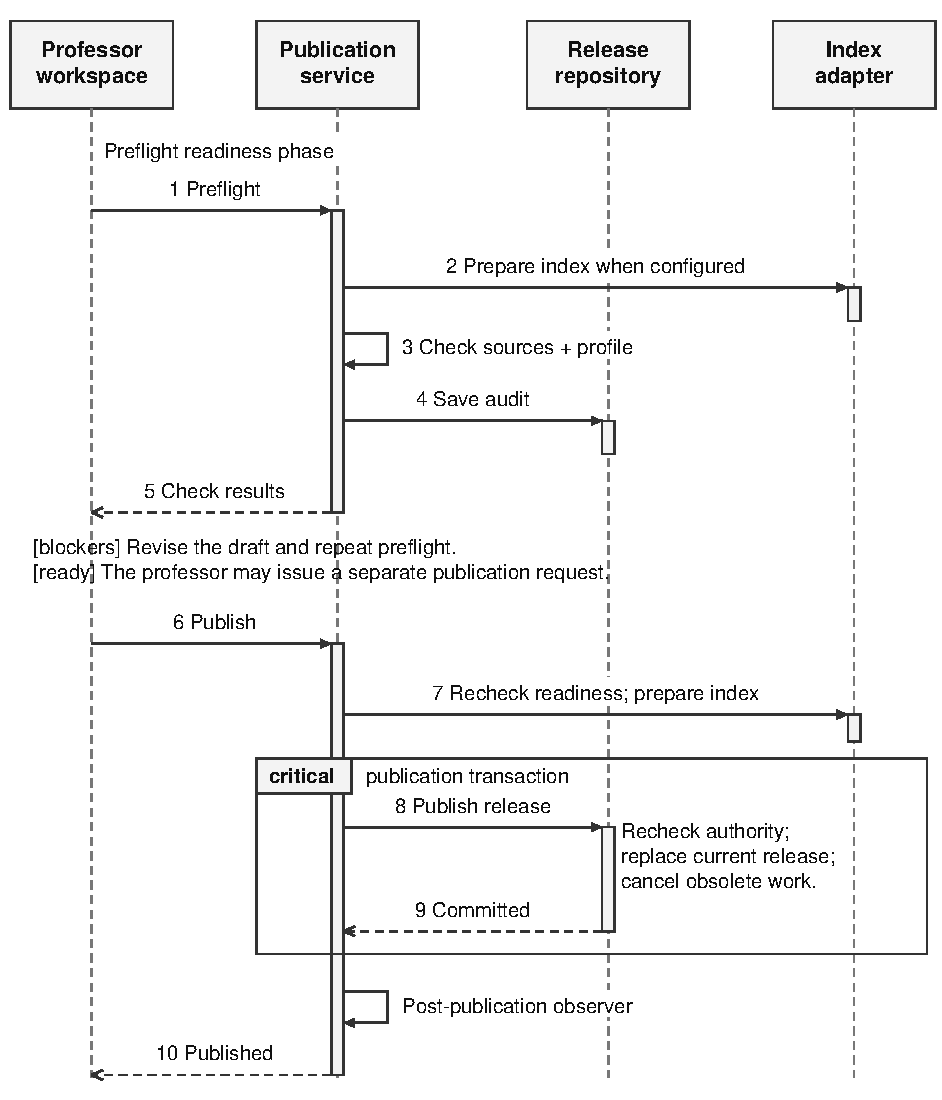
\includegraphics[width=\linewidth]{../../../reports/figures/course-twin-publication-sequence.pdf}
\caption{Preflight and publication interactions, with the release transaction shown explicitly.}
\label{fig:publication-detail}
\end{figure}
\FloatBarrier

\clearpage
\section{Software and Reproducibility}
\label{sec:software}
The retained component profile is
\path{research/05_evaluation/profiles/student-tutor-r1-local-final-v1.json}.
The project repository is \url{https://github.com/horiiiiii032929/digital-twin}
\cite{horinouchi2026digitaltwin}. It contains source code, synthetic evaluation
instruments and durable result summaries. Sensitive material and bulky generated
outputs are excluded. A repository URL identifies the project, not an immutable
experimental snapshot: reproduce a result using its recorded source revision,
dirty-state manifest, model configuration and dataset identifiers.

Table~\ref{tab:software} links the principal implementation dependencies to their
official documentation. Versions are taken from the current \path{uv.lock} and
\path{package-lock.json}, inspected on 6 September 2026; they are not attributed
to every historical run. Dynamic documentation was accessed on the same date.
Optional retrieval packages support comparisons and are not all selected runtime
components. The Qwen3 reranker adapter uses the prompt template published in the
\href{https://huggingface.co/Qwen/Qwen3-Reranker-0.6B}{Qwen3-Reranker model card};
that template is not a project contribution. 

\begin{table}[htbp]
\centering\small
\caption{Principal software dependencies (locked versions).}
\label{tab:software}
\begin{tabularx}{\linewidth}{@{}>{\raggedright\arraybackslash}L{0.22\linewidth}>{\raggedright\arraybackslash}Y@{}}
\toprule
Role & Software and official documentation \\
\midrule
API and validation & \href{https://fastapi.tiangolo.com/}{FastAPI} (0.141.1), \href{https://pydantic.dev/docs/validation/latest/get-started/}{Pydantic} (2.13.4). \\
Workflow and state & \href{https://docs.langchain.com/oss/python/langgraph/overview}{LangGraph} (1.2.11), SQLite checkpoint package (3.1.1), \href{https://www.sqlite.org/docs.html}{SQLite}, \href{https://aiosqlite.omnilib.dev/en/stable/}{aiosqlite} (0.22.1). \\
Model transport & \href{https://docs.litellm.ai/docs/}{LiteLLM} (1.97.0), \href{https://www.python-httpx.org/}{HTTPX} (0.28.1), \href{https://developers.openai.com/api/docs/guides/text}{OpenAI Responses API}. \\
Document processing & \href{https://pymupdf.readthedocs.io/en/latest/}{PyMuPDF} (1.28.2). \\
Web application & \href{https://react.dev/}{React} (19.2.8), \href{https://www.typescriptlang.org/docs/}{TypeScript} (7.0.2), \href{https://vite.dev/guide/}{Vite} (8.2.1), \href{https://tailwindcss.com/docs/installation/using-vite}{Tailwind CSS} (4.3.3). \\
Optional retrieval & \href{https://huggingface.co/docs/transformers/index}{Transformers} (5.15.1), \href{https://docs.pytorch.org/docs/stable/index.html}{PyTorch} (2.13.0), \href{https://www.sbert.net/}{Sentence Transformers} (6.0.0), \href{https://qdrant.github.io/fastembed/}{FastEmbed} (0.8.0). \\
Deployment & \href{https://docs.docker.com/compose/}{Docker Compose}, \href{https://caddyserver.com/docs/}{Caddy}; image configuration is recorded in the deployment files. \\
Testing & \href{https://docs.pytest.org/en/stable/}{pytest} (9.1.1), \href{https://vitest.dev/guide/}{Vitest} (4.1.10). \\
Dependency and report builds & \href{https://docs.astral.sh/uv/}{uv}, \href{https://tectonic-typesetting.github.io/en-US/}{Tectonic}, \href{https://ctan.org/pkg/natbib}{natbib}. \\
\bottomrule
\end{tabularx}
\end{table}

Diagram preparation was informed by Lek Hsiang Hui's IT5004 lectures 4,
``Requirements Analysis'' (PDF pp. 10--20, 54--58), and 5, ``Introduction to
Enterprise System'' (PDF pp. 7--19, 24--29), supplied as course materials;
the figures depict this project's implementation.

The repository README documents \verb|uv sync --locked --dev|,
\texttt{npm ci} and \texttt{npm run check}. The report README records the
Tectonic build command. Model identifiers and experimental selections are
versioned separately from library dependencies. 


\clearpage
\section{Development Lifecycle Traceability}
\label{sec:sdlc}
\begin{table}[htbp]
\centering\small
\caption{SDLC artifacts and acceptance conditions.}
\label{tab:sdlc}
\begin{tabularx}{\linewidth}{@{}L{0.17\linewidth}Y Y@{}}
\toprule Stage & Retained artifact and responsibility & Acceptance and next step \\\midrule
Requirements & Five user requirements in Table~\ref{tab:requirements}; approved project brief; \path{docs/quality-and-learning-plan.md}. Instructor defines knowledge, teaching policy and publication authority. & Walkthrough explains intended behaviour; instructor fidelity and real-course acceptance still require review. \\
Design & Architecture, response sequence and autonomy activity; \path{research/05_evaluation/profiles/}. Interfaces separate policy, providers and persistence. & Compare alternatives under shared conditions; retain unsuccessful choices and explicit fallback. \\
Implementation & Domain logic in \path{src/}, API in \path{services/}, interface in \path{apps/}; locked dependencies. & Trace requirements to executable boundaries; use \texttt{npm run check} for application checks.  \\
Verification & \path{tests/}; versioned cases and \path{research/05_evaluation/result-registry.md}. & Factual-support and teaching-alignment gates remain unresolved. Continuing-support simulations assess continuity under artificial events, not student learning. \\
Deployment & \path{docs/local-r1-runbook.md}; qualified configuration and rollback control. Operator starts API and workers with a shared persistent store. & Local qualification has a bounded environment. Confirm the exact profile, restore procedure and access controls before each deployment. \\
Operation and revision & Persisted goals, actions, outcomes and audit events; instructor dashboard and publication controls. & Observe failures, pause/withdraw when required, reproduce a defect, revise a candidate and rerun affected checks before updating the selected profile. \\
\bottomrule
\end{tabularx}
\end{table}

The goal-completion repair passed 72 focused service, component and audit tests.
The broader Python run and targeted rechecks verified 2,600 distinct tests;
this was not a single clean full-suite run after correction. The linked
\hyperref[study-H]{goal-completion record} preserves the initial failures,
local HTTPS permission issue, evaluation-runner classification repair and JUnit
records. The historical autonomy example is traced separately in
Appendix~\ref{sec:historical-autonomy}.

\clearpage
\section{Evidence Index}\label{sec:study-index}
Each link below opens the durable result summary, which records the configuration,
case counts, decision and limitations. The repository retains the full result
registry and individual attempts; raw execution settings, repeated approvals and
plan inventories are not reproduced in this report.
\begin{longtable}{@{}L{0.38\linewidth}L{0.57\linewidth}@{}}
\toprule Comparison & Evidence record \\ \midrule
\endhead
\phantomsection\label{study-A}Evidence-interface comparison & \href{https://github.com/horiiiiii032929/digital-twin/blob/main/research/05_evaluation/course-digital-twin-whole-system-architecture-round-2-001-results.md}{Result, method and limitations} \\
\phantomsection\label{study-B}Fresh factual comparison & \href{https://github.com/horiiiiii032929/digital-twin/blob/main/research/05_evaluation/final-cross-method-factual-confirmation-001-results.md}{Result, method and limitations} \\
\phantomsection\label{study-C}Action-planning comparison & \href{https://github.com/horiiiiii032929/digital-twin/blob/main/research/05_evaluation/successor-architecture-confirmation-005-001-results.md}{Result, method and limitations} \\
\phantomsection\label{study-D}Model-allocation comparison & \href{https://github.com/horiiiiii032929/digital-twin/blob/main/research/05_evaluation/successor-architecture-engine-comparison-006-001-results.md}{Result, method and limitations} \\
\phantomsection\label{study-E}Learner/timing simulation & \href{https://github.com/horiiiiii032929/digital-twin/blob/main/research/05_evaluation/successor-learner-timing-simulation-001-results.md}{Result, method and limitations} \\
\phantomsection\label{study-F}Revision comparison & \href{https://github.com/horiiiiii032929/digital-twin/blob/main/research/05_evaluation/independent-factual-revision-controls-001-fresh-v16-live-001-results.md}{Result, method and limitations} \\
\phantomsection\label{study-G}Live-model integration trial & \href{https://github.com/horiiiiii032929/digital-twin/blob/main/research/05_evaluation/final-profile-operational-dialogue-development-001-full-live-001-results.md}{Result, method and limitations} \\
\phantomsection\label{study-H}Goal-completion regression & \href{https://github.com/horiiiiii032929/digital-twin/blob/main/research/05_evaluation/goal-completion-scope-development-001-results.md}{Result, method and limitations} \\
\phantomsection\label{study-L1}Pipeline-scale test & \href{https://github.com/horiiiiii032929/digital-twin/blob/main/research/05_evaluation/factual-qa-v3-scale-completion-10000-001-results.md}{Result, method and limitations} \\
\phantomsection\label{study-L1c}Pipeline-test correction & \href{https://github.com/horiiiiii032929/digital-twin/blob/main/research/05_evaluation/factual-qa-v3-scale-completion-10000-001-analysis-correction-001-results.md}{Result, method and limitations} \\
\phantomsection\label{study-L2}Large product test & \href{https://github.com/horiiiiii032929/digital-twin/blob/main/research/05_evaluation/course-digital-twin-evaluation-program-011-results.md}{Result, method and limitations} \\
\phantomsection\label{study-L3}Whole-corpus regression & \href{https://github.com/horiiiiii032929/digital-twin/blob/main/research/05_evaluation/academic-factual-qa-open-10000-winner-regression-001-results.md}{Result, method and limitations} \\
\bottomrule\end{longtable}
The pipeline correction supersedes the original quality interpretation; neither
record is deleted. The goal-completion record compares old and corrected logic
and links the two arms. Its \href{https://github.com/horiiiiii032929/digital-twin/blob/main/research/05_evaluation/goal-completion-scope-review-audit-001-results.md}{scope audit}
explains the historical correction. The whole-corpus result contains the unresolved
numerical inconsistency discussed in Section~\ref{sec:large-regression}; its
headline percentage is not used as validated performance evidence.

\clearpage
\section{Planner Calculation and Evaluation Definitions}
\label{sec:planner-math}
This appendix expands the executable heuristic in
\path{src/digital_twin/student/planning_architectures.py}.
It describes the inspected implementation, not fitted educational parameters.
For an action $a$, let $p$ be the planning probability proxy, $u$ its uncertainty,
$z$ goal progress and $L$ the look-ahead depth (default two). With elapsed
observation time $t$ in days, spacing is $s=1-\exp(-t/3)$; when $t$ is absent,
the implementation uses $s=1$. The default adapter leaves $t$ absent.

\begin{align}
G(a)&=\min\{1,\ g_a(1-p)(0.5+0.5s)\},\\
O(a)&=\min\{1,\ o_a(0.5+0.5u)\},\\
F(a)&=\min\{1,\ 0.35L[G(a)+O(a)](1-z)\}.
\end{align}
The misconception bonus is $0.12$ for a hint/example or $0.04$ for a diagnostic
question when the inferred incorrect streak is at least two, otherwise zero.
Evidence risk is one when evidence is not ready, otherwise zero, with an
additional $0.05\max(0,k-2)$ for a check-in and clipping at one. Here $k$ is
the state card's evidence count; the default adapter populates it with the
number of supporting observation identifiers. The guarded
planner returns no action before scoring when its evidence-readiness check
fails; the risk term remains part of the shared forward-model interface.
No action has all terms and utility equal to zero.

\begin{table}[htbp]
\centering\small
\caption{Action constants used by the analytic forward model. Only
event-eligible and instructor-permitted actions are scored for a job.}
\begin{tabularx}{\linewidth}{@{}Yrrr@{}}
\toprule Action & $g_a$ & $o_a$ & $I(a)$ \\\midrule
Diagnostic question & 0.05 & 0.28 & 0.03 \\
Hint or example & 0.18 & 0.12 & 0.04 \\
Approved-source recommendation & 0.12 & 0.08 & 0.04 \\
Retrieval practice & 0.24 & 0.24 & 0.05 \\
Schedule follow-up & 0.02 & 0.03 & 0.02 \\
In-app check-in & 0.03 & 0.05 & 0.08 \\
Progress summary & 0.04 & 0.02 & 0.04 \\
Professor insight draft & 0.01 & 0.00 & 0.01 \\
No action & 0.00 & 0.00 & 0.00 \\
\bottomrule
\end{tabularx}
\end{table}

For the worked calculation in Section~\ref{sec:planning}, a hint has
$G=0.09$, $O=0.08$, $F=0.119$, $B=0.12$, $R=0$ and $I=0.04$.
The sum is $0.325$. The diagnostic question has $G=0.025$,
$O\approx0.186667$, $F\approx0.148167$, $B=0.04$, $R=0$ and $I=0.03$,
giving approximately $0.267167$. This is a calculation from constants and a
declared state, not an invented empirical case.

The component evaluation uses a different quantity. If the hidden instrument
assigns action value $v_i(a)$ in context $i$, the selected action is $\hat a_i$
and $N$ is the number of contexts, then
\begin{equation}
\overline v=\frac1N\sum_i v_i(\hat a_i),\qquad
\overline r=\frac1N\sum_i\left[\max_a v_i(a)-v_i(\hat a_i)\right].
\end{equation}
The \hyperref[study-C]{action-planning comparison}'s utility improvement is $0.004805$, with paired 95\% interval
$0.003065$--$0.006760$ over 1,000 contexts. Its preferred-label difference
is $-0.01$, with interval $-0.022$--$0.001$. Utility, preferred action and
the runtime score therefore answer different questions. The synthetic action
values and the model's internal prediction do not constitute observed learning.

\clearpage
\section{Synthetic Teaching Profiles and Saved Responses}\label{sec:profile-examples}
A teaching profile specifies tone, explanation depth, examples, misconception
handling and the sequence of assistance. A Socratic policy can prefer an initial
question or a hint; an explanatory policy can permit a direct explanation.
The synthetic profiles used in the saved dialogue trial expose eight fields
(Table~\ref{tab:profile-fields}). Their values enter the approved teaching-context
candidate, where the service supplies them together with the current question,
permitted evidence and dialogue state. A profile change therefore needs a new
reviewed binding; a student message is not allowed to replace that configuration.

\begin{table}[htbp]
\centering\small
\caption{Teaching fields in the live-model integration trial's synthetic profiles.}
\label{tab:profile-fields}
\begin{tabularx}{\linewidth}{@{}L{0.24\linewidth}YY@{}}
\toprule Field & Socratic configuration & Explanatory configuration \\\midrule
Tone / depth & Patient and reflective; concise & Direct and precise; detailed \\
Explanation structure & Diagnostic question, attempt, one hint & Explanation, example, understanding check \\
Example preference & Learner constructs an example & Concrete non-assessed example \\
Misconception handling & Contrast question before correction & Explain correction, then apply it \\
Integrity limits & Require an attempt; no assessed-work solutions & Same restriction \\
Help ladder & Question, hint, guided explanation & Explanation, worked example, application question \\
Outreach policy & Reflective lead; contrast alternatives & Direct lead; apply the evidence \\
\bottomrule
\end{tabularx}
\end{table}
Source: \path{scripts/teaching_profile_responsiveness_packet.py}, used by the
operational dialogue runner. Tone and depth are separate fields shown together
for compactness. 

Table~\ref{tab:worked-example} uses saved outputs from the 24-history operational
trial. These are separate synthetic contexts, not a controlled comparison of the
effect of changing a single profile.

\begin{table}[htbp]
\centering\small
\caption{Saved configuration-to-response examples from the live-model integration trial.}
\label{tab:worked-example}
\begin{tabularx}{\linewidth}{@{}L{0.20\linewidth}Y@{}}
\toprule Context & Stored output and interpretation \\\midrule
Socratic; first turn & Student: ``How does slot seal work in this course protocol?'' Tutor: ``For `How does slot seal work', what is your current explanation, and which step are you unsure about?'' The system elicits an attempt, but the question remains generic. \\
Explanatory; day 30 & Student asks how lantern check works. Tutor: ``lantern check sends a probe to each station'' and ``marks a station unavailable after two consecutive unanswered probes''. The reply supplies the source rule; repeated extraction does not establish personalized progression. \\
Proactive support & All 16 reviewed check-ins used a generic wrapper around an entire synthetic source card. Authority checks permitted delivery; the effect of these messages on students was not measured. \\
\bottomrule
\end{tabularx}
\end{table}
The source record is \path{research/05_evaluation/dialogue-full-live-001-assistant-findings.json};
its finding identifiers F21 (Socratic example) and F03 (explanatory example) retain the history, day, student input, response and diagnostic finding.
The operational trial is reported in Section~\ref{sec:provider-study} and indexed
in Appendix~\ref{sec:study-index}.


\clearpage
\section{Historical Multi-concept Trial and Correction}\label{sec:historical-autonomy}
\textbf{Recorded example.} In the saved deterministic fast-learner history
(seed 3101, Bayesian-style simulator), the first day contains a diagnostic
question and a hint. Before the next recorded student turn, an
\texttt{incomplete-objective} event produces an in-app check-in: the goal still
requires assessed evidence, and the deterministic event rule selects that
permitted action. The saved opportunity, action and delivery-message identifiers
link the decision to its persisted effect and source citation. Subsequent turns
produce further learner-state revisions; the day-15 restart check retains an
identical state hash. By the end, the token-bucket concept has eight correct and
four incorrect assessments, illustrating why a delivered check-in is not itself
proof of mastery. This is one operational trace, not evidence that the check-in
caused those later outcomes. Its source is the \href{https://github.com/horiiiiii032929/digital-twin/blob/main/research/05_evaluation/governed-full-autonomy-v2-1-multi-concept-confirmation-025-results.md}{historical multi-concept result}; the sanitized trace is retained in
\path{research/06_reports/final/professor-reader-review.md}.


\subsection{Original Reported Simulator Outcomes}
For the autonomous-support question, the deterministic longitudinal study compared 72 histories in 36 matched pairs.
A pair shares the specified learner scenario and seed, with autonomous support
in one history and reactive-only support in the other. This is a comparison
within the simulator, not a randomized study of students.
It exercised 30 virtual days of tutoring and intervention logic without external
LLM calls. Simulated mastery averaged 0.365 with autonomous support and 0.332
with the reactive control; the paired difference was 0.0324, with a 95\% interval
of 0.0040--0.0617. For pair $k$, let $m_k^{A}$ and $m_k^{R}$ be final simulated mastery under
autonomous and reactive support, respectively. Each history's mastery summarizes
its simulated concepts on a zero-to-one scale. The paired mean difference is
\begin{equation}
\overline{\Delta m}=\frac{1}{36}\sum_{k=1}^{36}(m_k^{A}-m_k^{R})=0.0324.
\label{eq:mastery-difference}
\end{equation}
This is 3.24 percentage points on the simulator's scale. It is computed from
unrounded paired values, so subtracting the displayed rounded means need not
reproduce it exactly. Its interval resamples the paired differences. Both the
means and their difference follow the simulator's learning and forgetting rules;
they are not measured student learning gains.

Predictive area under the receiver operating characteristic curve (AUROC) summarizes how well the previous learner-state estimate ranks
later correct above incorrect simulated attempts. A value of 0.5 gives no ranking
advantage; 1 indicates perfect ranking. The reported 0.466, averaged over histories with both outcomes, therefore
provides little evidence of useful prediction. A simulated intervention is labelled
wasted when its recipient is already at the mastery threshold or is unreceptive.
The reported 32.9\% is an average of per-history wasted-delivery rates, rather
than a human judgment of whether a message helped. These diagnostics reveal
weaknesses that successful consent and restart checks cannot detect.


\paragraph{Later interpretation correction.}
These numbers describe the original multi-concept implementation. The subsequent
goal-scope audit found ten unsupported completed goals among 22 completions
across eight histories, even though the concept-assessment gates had passed.
The old paired mastery difference is therefore retained as a historical
simulator outcome, not evidence for the corrected lifecycle or real learning.
The \hyperref[study-H]{goal-completion regression} uses new seeds on the same exposed concepts and reports its own
paired results; it does not overwrite or rescore the historical trial.





\end{document}
